\documentclass[../thesis.tex]{subfiles}
% Separate preamble for this subfile. This preamble is loaded last, so one can override various functions before \begin{document}

% Better comment extension for Vscode colors these comments differently
% Normal comment color
% * Important information
% ! ALERT
% ? Question
% TODO stuff to do
% // This is strikethrough


\begin{document}

\mycomment{

Den tiden som gjennstår:


Jo høyere dimensjon vi får jo mer eksotisk kan disse tilingene bli. Står noe referanser til i paperet. 
Keller hadde en teori om at enhver tiling må være av den typen -- (Se for deg enhetskuben i 2D)
enhver tiling nødvendigvis medføre at,
alle tiles har en full felles kant med en annen tile

i 2D gjelder det her med at man har to kanter hvor man har en full felles kant (med den over og den under)


i 1D har man ingen sidekant, det er et punkt
men poenget er at i veldig høye dimensjoner så kan tilingene bli mer eksotiske, og et utrykk for det er at du ikke trenger å ha en full kant med noen som helst annen tile
dimensjon > 7
}




%!  Uformell definisjon av hva vi mener med det
%* Figurer og eksempler, 1 eller 2D, trenger ikke gå opp til 3D.
%* Det må inn noen figurer som gjør at når det kommer til tilings, så finnes det noen mengder som bare tiler med translasjoner, og noen mengder som vil krevet at man roterer eller speiling, og at vi skal holde oss til de som er kun med translasjon.

Informally, to tile refers to the process of covering some surface with objects. These objects are called tiles and come in a variety of shapes and sizes. When we are tiling, we essentially place copies of the tile next to each other in a systematic way, intending to leave no gaps and no overlaps between the tiles. The resulting tiling can be as simple as the one shown in \cref{fig:tiling_one} where we have used a single tile, the unit square, to tile the plane, or as complex as \cref{fig:tiling_two} where we have used four different tiles to tile the plane. The first is an example of what is known as a \emph{monohedral tiling} in which all tiles are congruent \cite[p. 20]{grunbaumTilingsPatterns1987}, and the latter is an example of a Penrose tiling which are well known for being non-periodic \cite{penrosePentaplexityClassNonPeriodic1979}. %* PAge 535 har også penrose tilings
% non-periodic tiling, meaning that there is no period parallelogram \SigridChange{KORT FORTALT}. 




\begin{figure}[h!]%h!
    \centering
    \begin{subfigure}{.47\textwidth}
        \centering
        %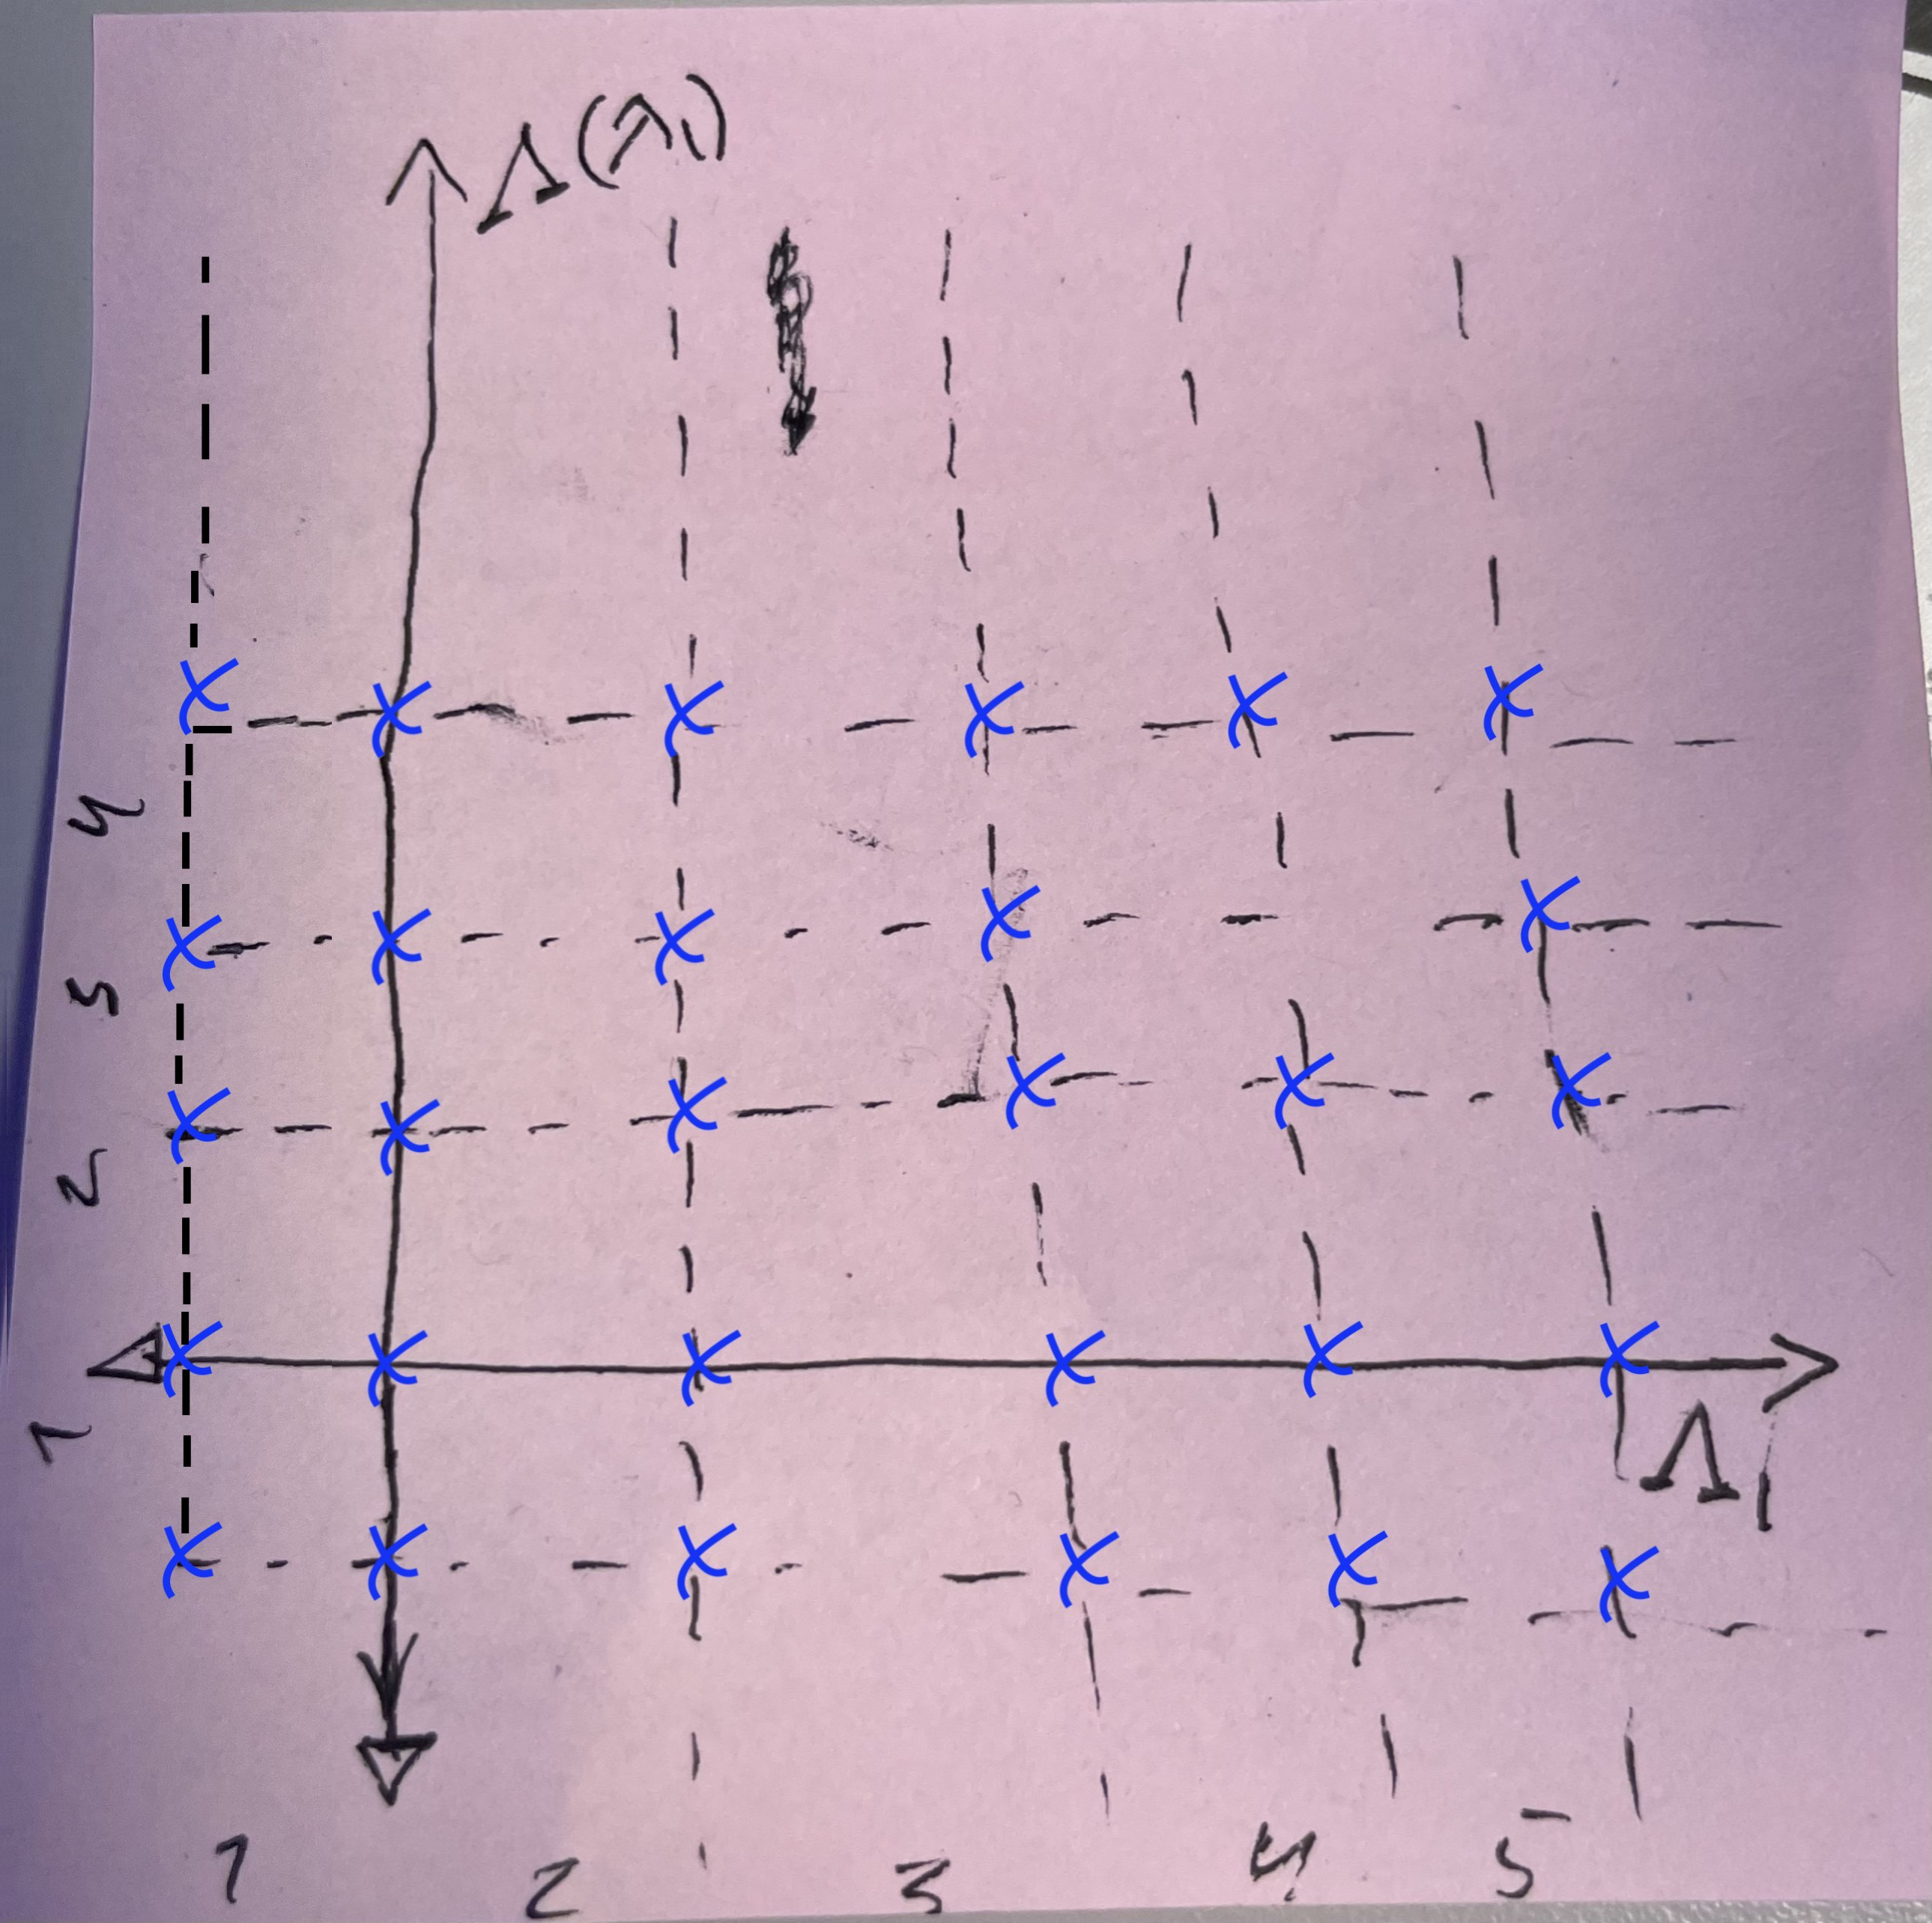
\includegraphics[width=0.9\linewidth]{spec_no_shift.jpg}
        %* Figure 1
        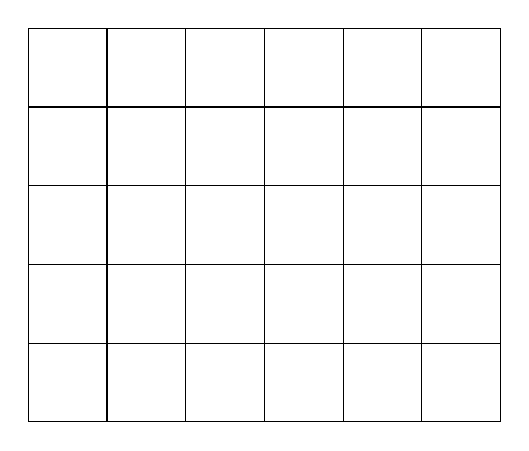
\begin{tikzpicture}[scale=1]
            % Define the tile
            \def\tile{
              % Draw the unit square
              \draw (0,0) rectangle (1,1);
            }
          
            % Draw the tiling pattern
            \foreach \x in {0,1,2,3,4,5}{
              \foreach \y in {0,1,2,3,4}{
                \pgfmathsetmacro{\shiftX}{\x} % Set horizontal shift
                \pgfmathsetmacro{\shiftY}{\y} % Set vertical shift
                \begin{scope}[shift={(\shiftX,\shiftY)}]
                  \tile % Draw the tile
                \end{scope}
              }
            }
        \end{tikzpicture}
        %* —————————————————
        \caption{Lattice tiling}
        \label{fig:tiling_one}
    \end{subfigure}\quad
    \begin{subfigure}{.47\textwidth}
        \centering
        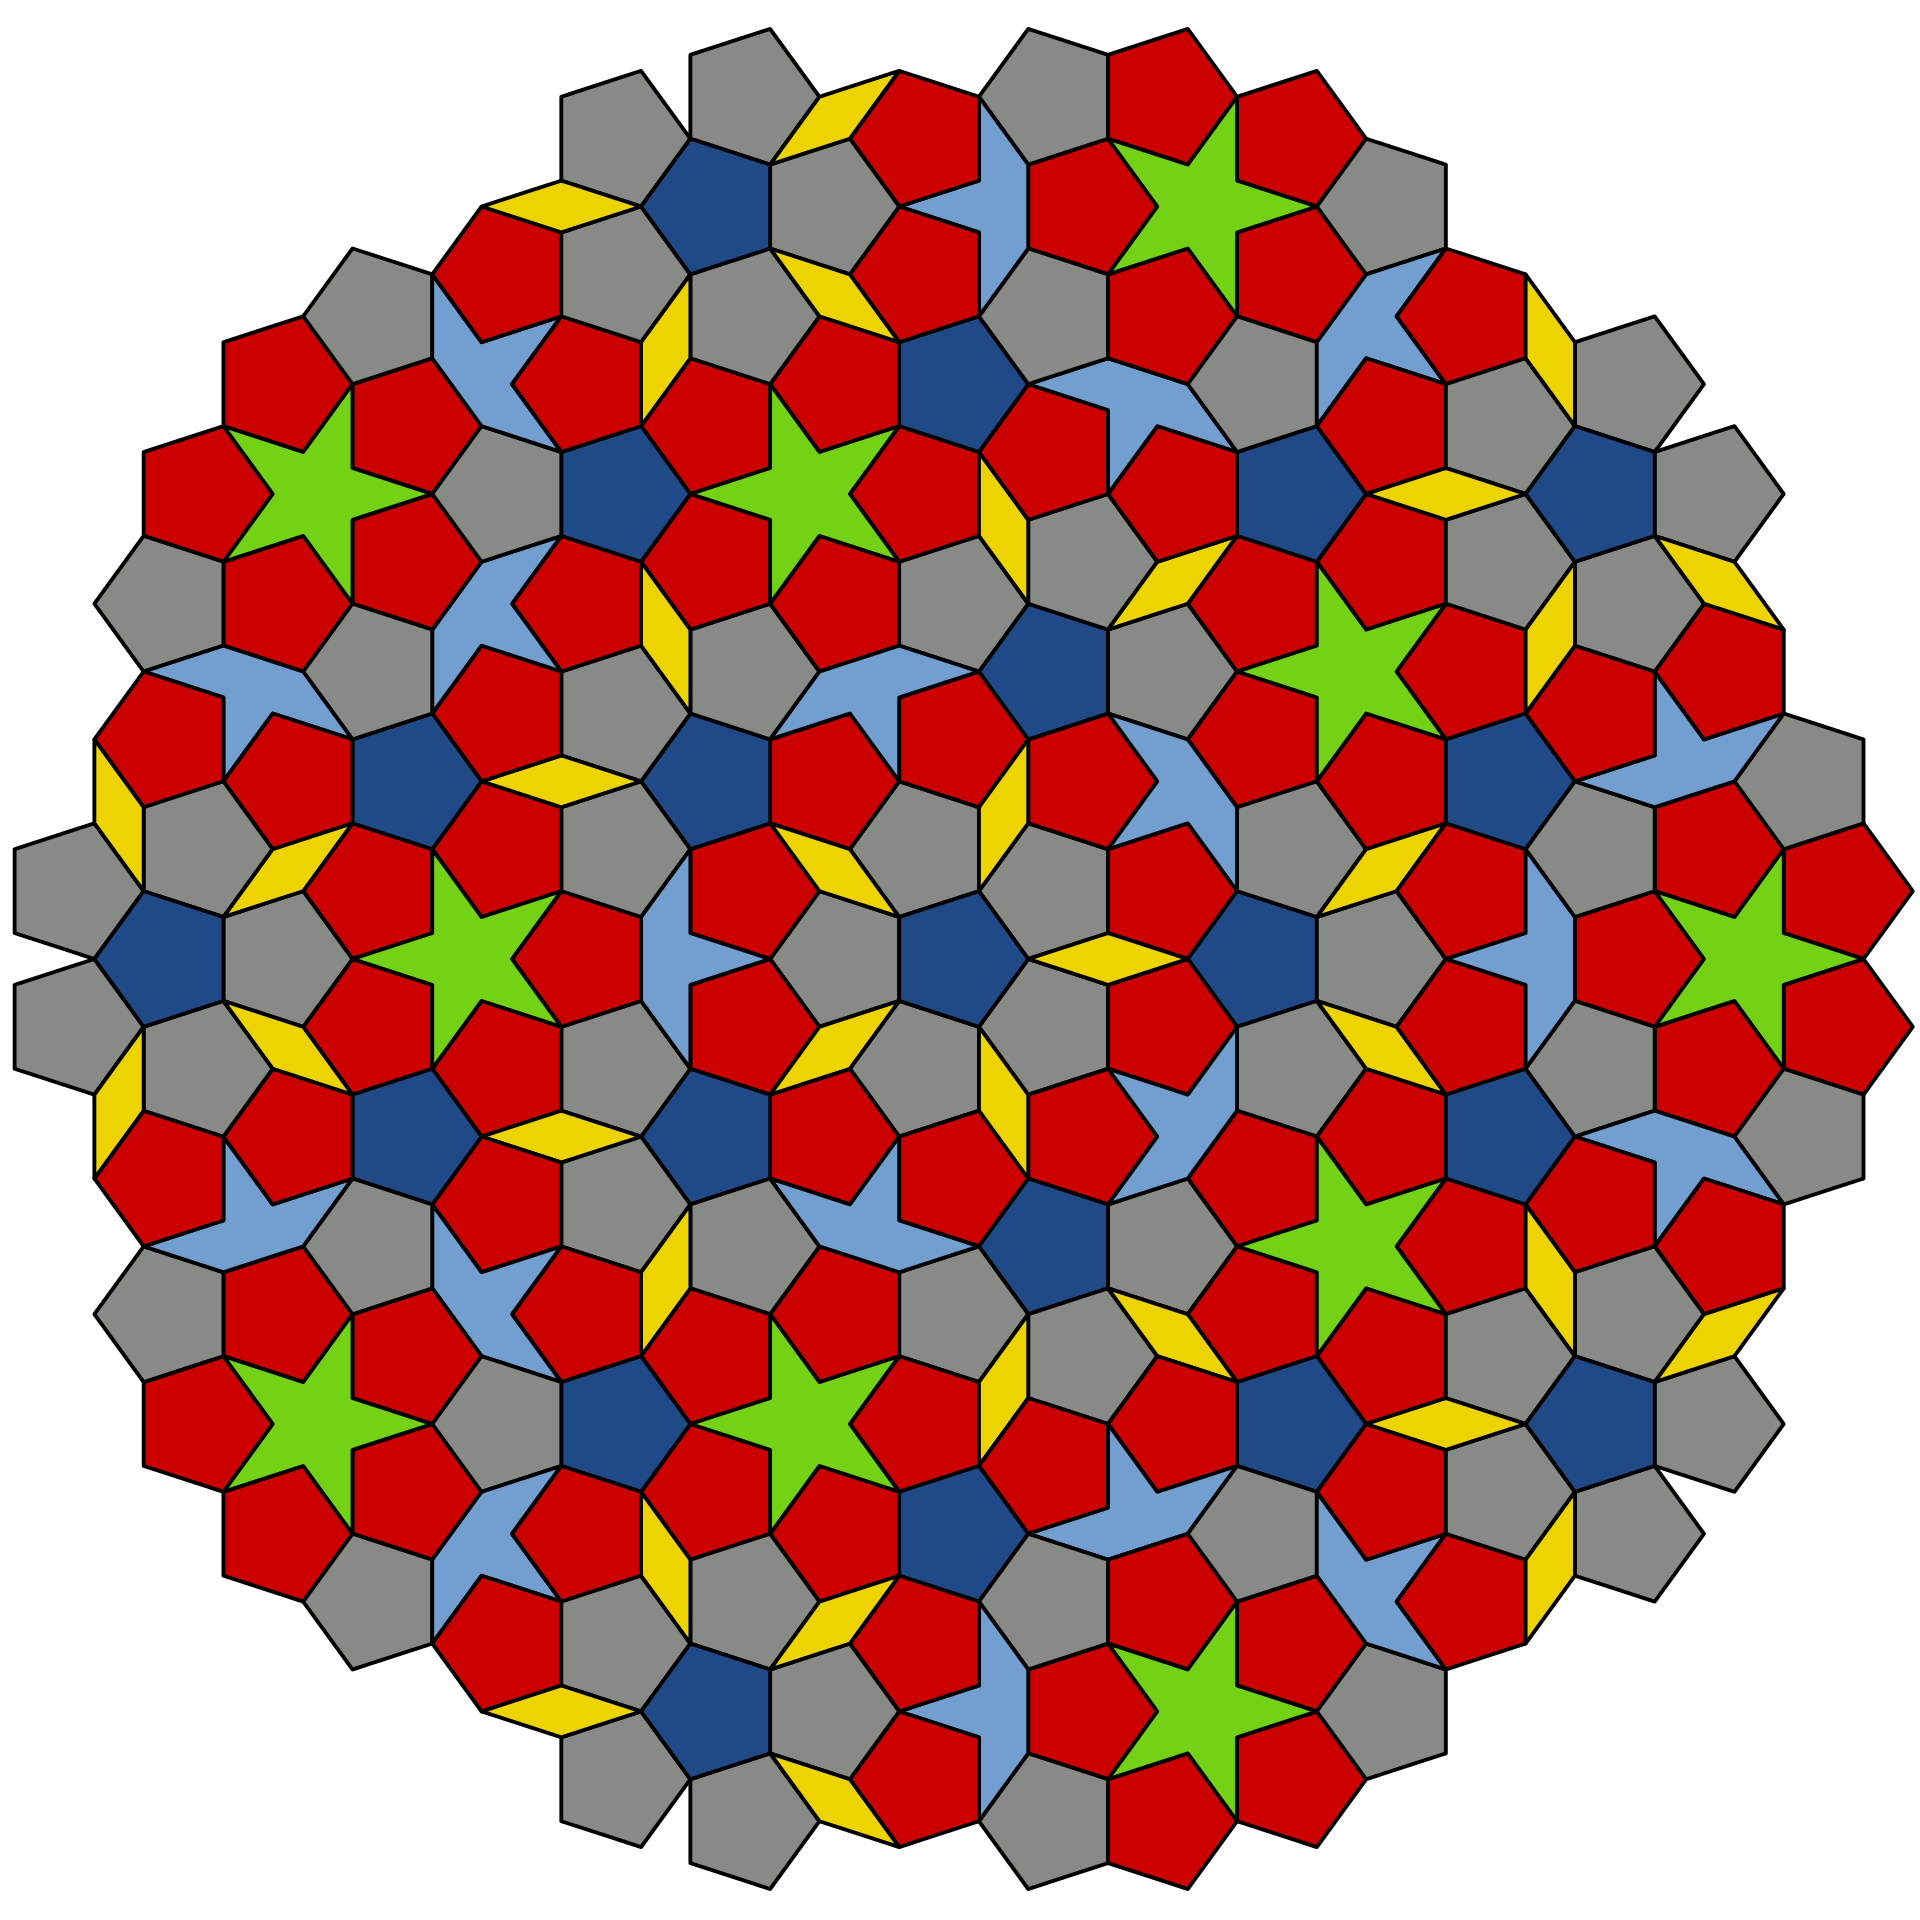
\includegraphics[width=0.87\linewidth]{Penrose_Tiling_.png}
        \caption{P1 Penrose tiling \cite{inductiveloadP1TilingUsing}}
        \label{fig:tiling_two}
    \end{subfigure}
    \caption{Two contrasting tilings of the plane to emphasize the range of complexity. \cref{fig:tiling_one} shows a simple monohedral tiling, and \labelcref{fig:tiling_two} shows an intricate, non-periodic tiling using four different tiles. The coloring in the latter is used to distinguish the tiles more easily and highlight the three \emph{matching rules} for the pentagonal tiles, the only ones with different colors for the same shape. Matching rules are needed in order to tile aperiodically \cite{penrosePentaplexityClassNonPeriodic1979}.}
    \label{fig:tilings_one_two}
\end{figure}

% Penrose goes into the details of these in his paper 

\mycomment{  %! Block comment
The lattice tiling in \labelcref{fig:tiling_one} has fewer tiles and lacks variety compared to Penrose's original aperiodic tiling.

Two tilings of the plane to emphasize the contrast between monohedral tilings and an intricate tiling
Two tilings of the plane emphasize the contrast from monohedral tilings to more intricate tilings, such as the Penrose tiling in Fig. 

Two contrasting tilings of the plane between a monohedral tiling in \cref{fig:tiling_one} and more intricate tilings such as the Penrose tiling in \cref{fig:tiling_two} 

In contrast to the simple monohedral tiling shown in \cref{fig:tiling_one}, the Penrose tiling in \cref{fig:tiling_two} and other intricate tilings provide contrasting examples of tilings on the plane.
In contrast to the simple monohedral tiling shown in \cref{fig:tiling_one}, the Penrose tiling in \cref{fig:tiling_two} is a contrasting example of a more intricate tiling of the plane. 
In contrast to the simple monohedral tiling shown in \cref{fig:tiling_one}, the Penrose tiling in \cref{fig:tiling_two} is an example of a more intricate tiling of the plane. 

Two contrasting tilings of the plane to emphasize the stark difference between a simple monohedral tiling in \cref{fig:tiling_one} and more intricate tilings such as the Penrose tiling in \cref{fig:tiling_two}.
Two contrasting tilings of the plane to emphasize the stark difference between a simple monohedral tiling in \cref{fig:tiling_one} and a more intricate tiling in \cref{fig:tiling_two} which is non-periodic and uses four tiles. 

To emphasize the stark difference between a simple monohedral tiling in \cref{fig:tiling_one} and a more intricate tiling in \cref{fig:tiling_two} which is non-periodic and uses four tiles, we present two contrasting tilings of the plane.

Two contrasting tilings of the plane to emphasize the range of complexity. \cref{fig:tiling_one} shows a simple monohedral tiling, and \cref{fig:tiling_two} shows an intricate, non-periodic tiling using four different tiles. 
} 

Another interesting monohedral tiling is given in \cref{fig:tiling_three}. This is an example of an Escher lizard tiling \cite{kolountzakisTilingsTranslation2010}. Note that in comparison to the square tilings in \cref{fig:tiling_one}, there is important to highlight a fundamental difference between the square and lizard tilings. In the latter, one needs to rotate the lizard tile in order to cover the entire surface. In addition to translation and rotation, one can also have reflections. Although not shown in any figure, it is worth mentioning for completeness.  
\SigridComment{I am concerned if the last sentence is something worth mentioning or that there probably are other symmetries in higher dimensions that make it not correct in terms of "completeness"}
% However, it is essential to highlight a fundamental difference between the square tilings in \cref{fig:tiling_one} and the lizard tilings in \cref{fig:tiling_three}. In the latter, one needs to rotate the tile in order to cover the entire surface. 

\mycomment{ %! If we bring in reflection —— We don't ——
However, it is important to highlight a fundamental difference between the square tilings in \cref{fig:tiling_one}, the lizard tilings in \cref{fig:tiling_three}, and the BLABLA tilings in \cref{fig:tiling_four}. Each represents a way to cover the entire surface exclusively using either translation, rotation, or reflection in that order.  
% OPTION 1: Delete "in that order" and write: Meaning square tilings need only translation to cover the entire surface, lizard tilings need only rotation, and BLABLA only needs reflection.
% OPTION2: It means square tilings can cover the entire surface using translation, lizard tilings need only rotation, and BLABLA only needs reflection. 
% OPTION 3: The first, \cref{fig:tiling_one}, can tile the surface using translation only, \cref{fig:tiling_three} can tile using rotation only, and \cref{fig:tiling_four} can tile using reflection only.
}
%  https://www.wikiart.org/en/m-c-escher/flying-fish    
%  https://www.wikiart.org/en/m-c-escher/lizard-1} 



\begin{figure}[t]%h!
    \centering
    \begin{subfigure}{.47\textwidth}
        \centering
        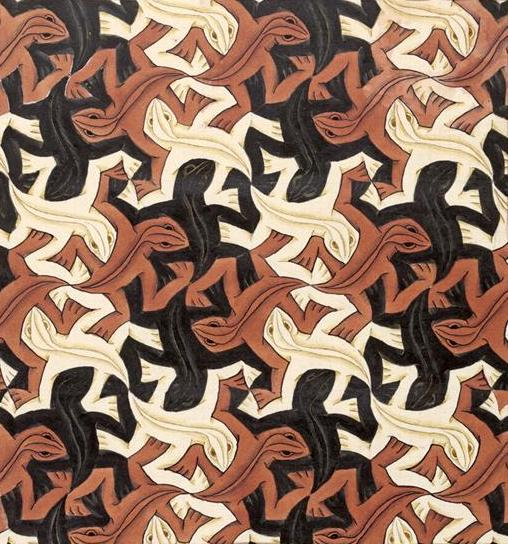
\includegraphics[width=0.9\linewidth]{lizard-1.jpg}
        \caption{Lizard}
        \label{fig:tiling_three}
    \end{subfigure}\quad
    \begin{subfigure}{.47\textwidth}
        \centering
        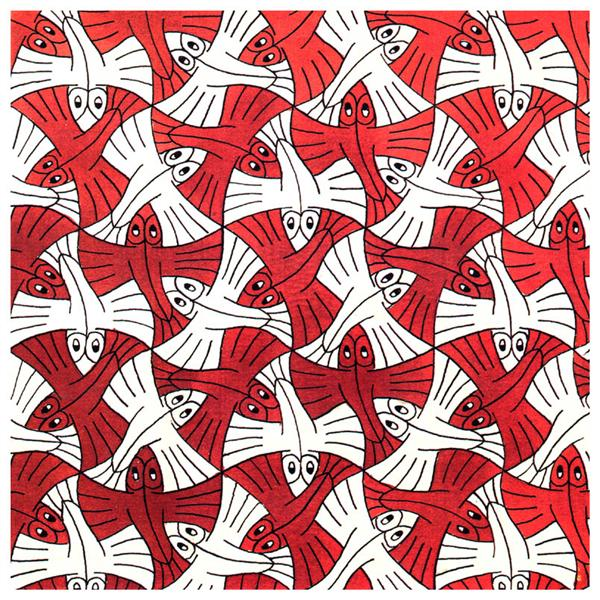
\includegraphics[width=0.9\linewidth]{flying-fish.jpg}
        \caption{Flying fish}
        \label{fig:tiling_four}
    \end{subfigure}
    \caption{Text}
    \label{fig:tilingsss_two}
\end{figure}

However interesting the Penrose and Escher tilings appear, we will only focus on tilings of $\R^d$ by translation and using only the unit cube as our tile. Considering only cube-tilings might seem simple initially, but we will see that as we increase the dimension, we get increased flexibility and more complex tilings. It turns out that in higher dimensions, highly exotic and counterintuitive cube tilings exist \cite{iosevichSpectralTilingProperties1998}. The fact that these exotic tilings exist in the first place is surprising in light of Keller's theorem. / The fact that this kind of tiling exists in the first place is surprising in light of Keller's theorem \cite{iosevichSpectralTilingProperties1998}%This is Perhaps surprising in light of Keller's theorem. 
%! Orginalpaperet har både conjecture og theorem? Hvis dette stemmer, endre andre citation til orginalpaperet. Hvis det ikke stemmer, flytt citation for dette avsnittet helt sist, for keller er hentet fra det paperet. 


%* VELG en 
For the proof of the theorem, the reader is referred to \cite{iosevichSpectralTilingProperties1998}. 
Although we will not prove it here, the reader is referred to a paper by Pedersen and Iosevich for proof \cite{iosevichSpectralTilingProperties1998}. 

The theorem was initially presented in \cite{ott-heinrichkellerUberLuckenloseErfullung1930} and proved by his student in PER.


%\begin{theorem}\label{thrm:keller_tiling} %* Orginale keller fra paperet til iosovich og pedersen
%    Given a discrete subset $T\subset \R^d$. If $T$ is a tiling set for $\Omega$, then given any pair $\lambda, \lambda' \in T$ such that $\lambda\neq\lambda'$, there exists a $j\in \braq{1,\dots,d}$ so that $\bral{t_j -t_j' } \in \N$
%\end{theorem}
\begin{theorem}[Keller's Theorem]\label{thrm:keller_tiling}
    Let $\Lambda \subset \R^d$ be a discrete subset. If $\Lambda$ is a tiling set for the unit cube $\bras{0,1}^d$, then given any pair $\lambda, \lambda' \in \Lambda$ such that $\lambda\neq\lambda'$, there exists a $j\in \braq{1,\dots,d}$ so that $\lambda_j -\lambda_j' \in \intnozero$.
\end{theorem}
%* Viktig, må inn en bit her om 
%* som en konsekvens av Kellers theorem så får vi nå akkurat den samme formen på disse tilings settene 
%* de må ligge inneholt i akkurat de samme typene mengder, og de kan ikke være ekte mindre for da får vi ikke oppfylt tiling kravet mitt.



%! OPTIONAL IF TIME: The proof of Keller's theorem is in CREF section 3.1. 



In the same paper, Keller conjectured the following. %* Keller conjectured that
%* ELLER NOE SÅNT.  # OVERGANG intro, historie

\begin{conjecture}
    All tilings of $\R^d$ by translations of the unit cube contain two cubes that share an entire $(d-1)$-dimensional face.
\end{conjecture}

%! Vurder å skrive om hele avsnittet under her 
%* Known to be true... d<=7, but in fact false when d>7...

If the dimension is two, the squares share an edge; if the dimension is three, they share a face. This conjecture is now known to be true for all $d\leq 7$ after it was recently proven true in dimension seven \cite{brakensiekResolutionKellerConjecture2020}. % and we can still have quite the exotic and counter-intuitive tiling. %Worth emphasizing is the fact that we lack a method for determining whether a tile is the prototile of a monohedral tiling 

%* Det Sigrid vil ha med i Grønt
If $d>7$ the conjecture is false. 

%* Det som er viktigst å si i fra om det er følgende
%* Det er at denne conjecturen støtter ikke opp om det at man skal ha eksotiske tilings, snarere tvert i mot. Den gir en indikasjon på rigiditet her.
%* Men nettopp fordi vi vet at den er usann når d>7 så dukker disse eksotiske greiene opp

%* Derfor blir følgende er ikke helt riktig:
%* "One indicator of this characteristic follows from Keller's conjecture \cite{ott-heinrichkellerUberLuckenloseErfullung1930}."

%* Det at conjecturen er usann for d>7 finnes det gode kilder på. For å kaste lys på at de kan være eksotiske så er det det at de er usant over 7 som er det relevante her. 


%? info
%? Keller's paper inneholder mest ss. begge resulatene, så om Sigrid hadde vært Keller så hadde jeg tenkt følgende
%* Hvis jeg kan vise at jeg alltid har denne heltalls-differansen så er det naturlig å anta at jeg kan styrke denne mikovsky conjecturen.
%* Dette er fordi  han viser theoremet uavhengig av om det er en lattice eller ikke





%* ———————————————————————————— Tilings ——————————————————
%* Tenk overgang, vurder intro med non overlappings og coverings, litt uformelt, ingen def, dvs det fra gammelt med gammel struktur og så lede over til vår def
In defining tilings formally, we use indicator functions... 

CITATION, en, ikke begge \cite{kolountzakisTilingsTranslation2010} \cite{kolountzakisStudyTranslationalTiling2003}. 


Rather than defining tiling in terms of a non-overlapping covering of the space, we will instead define tiling by the indicator function, using little of our geometric intuition \cite{kolountzakisTilingsTranslation2010} \cite{kolountzakisStudyTranslationalTiling2003}. 

\begin{definition}[Tiling set]
    Let $\Omega \subset \R^d$ be a subset with nonzero measure, and consider a \SigridChange{discrete (or just a set?)} set $\Lambda \subset \R^d$. If
    \begin{equation}\label{eq:tiling_set}
        \sum_{\lambda \in \Lambda} \indicator{\Omega}{x-\lambda} = 1, \text{\space} a.e. \quad x \in \R^d,
    \end{equation}
    then $\Omega$ is called a \emph{tile}, and $\Lambda$ is called a \emph{tiling set} for $\Omega$. We say that $(\Omega, \Lambda)$ is a \emph{tiling pair}.
\end{definition}
In other words, we can also say that $\Omega$ \emph{tiles $\R^d$ by translation}, or that $\Omega$ is a \emph{tiling} of $\R^d$. 

%* Etterpå kunne vi vurdert å nevne at det er mulig å tile med funksjoner, kommentar om dette på side 11




%* —————————————————— en dimensjon
If we now restrict our attention to the unit cube in d-dimensions, Keller's theorem immediately gives the following for $d=1$. In dimension one, the unit cube is simply the unit interval $I = \bras{0,1}$. 

\begin{lemma}\label{lem:tiling_unit_1d}
    The set $\Lambda = \Z +\alpha$ for some value $\alpha\in \R$ constitutes a tiling set for the unit cube.
\end{lemma}
%\begin{theorem}  %* Bruker alle elementene i T for å flytte på I, da dekker vi hele $\R$.  
%    Let $\Omega = I$. If $T=\Z$, then $T$ is a tiling set for $I$.
%\end{theorem}

\begin{proof}  % This follows directly from \cref{thrm:keller_tiling}. Take $\lambda, \lambda' \in \Lambda$. 
    

\end{proof}

%! Dette må skrives
The proof of \cref{lem:tiling_unit_1d} follows directly from \cref{thrm:keller_tiling} as it tells us directly that there must be an integer distance between two distinct points $\lambda,\lambda' \in \Lambda$ in a tiling set for $I$ where $\Lambda \subset \Z +\alpha$. Note that the value $\alpha$ cancels out. In addition, we must have equality, that is, $\Lambda = \Z +\alpha$. Otherwise, we would not satisfy \labelcref{eq:tiling_set} since we would have an entire interval with measure not equal to one.

Increasing the dimension by one 








%! New structure to be written in above

%* Gammelt
%* denne introen til tilings kan vurderes å droppes for T(\Lambda) ville da vært en tiling OG IKKE et tiling set
To begin, given a subset $\Omega$ of $\R^d$ and a discrete set $\Lambda$ of $\R^d$, we denote by $T(\Lambda)$ the set of translates 
\begin{equation*}
    T(\Lambda) = \braq{\Omega+\lambda : \lambda\in \Lambda},
\end{equation*}
where $\Omega + \lambda$ is the translate of $\Omega$ by the vector $\lambda$. That is the set
\begin{equation*}
    \Omega + \lambda = \braq{\omega + \lambda : \omega \in \Omega}.
\end{equation*}
Rather than defining tiling in terms of non-overlapping and covering of the space, we will instead define tiling in the Fourier domain, using little of our geometric intuition \cite{kolountzakisTilingsTranslation2010} \cite{kolountzakisStudyTranslationalTiling2003}. 
%* ———————






\SigridComment{opppskalering til 2D}
\SigridComment{usikker på strukturen og hvordan jeg skal skrive og forklare inneholdet her}

samme figur som for spektra, men her med tilings



\begin{figure}[t!]%h!
    \centering
    \begin{subfigure}{.47\textwidth}
        \centering
        %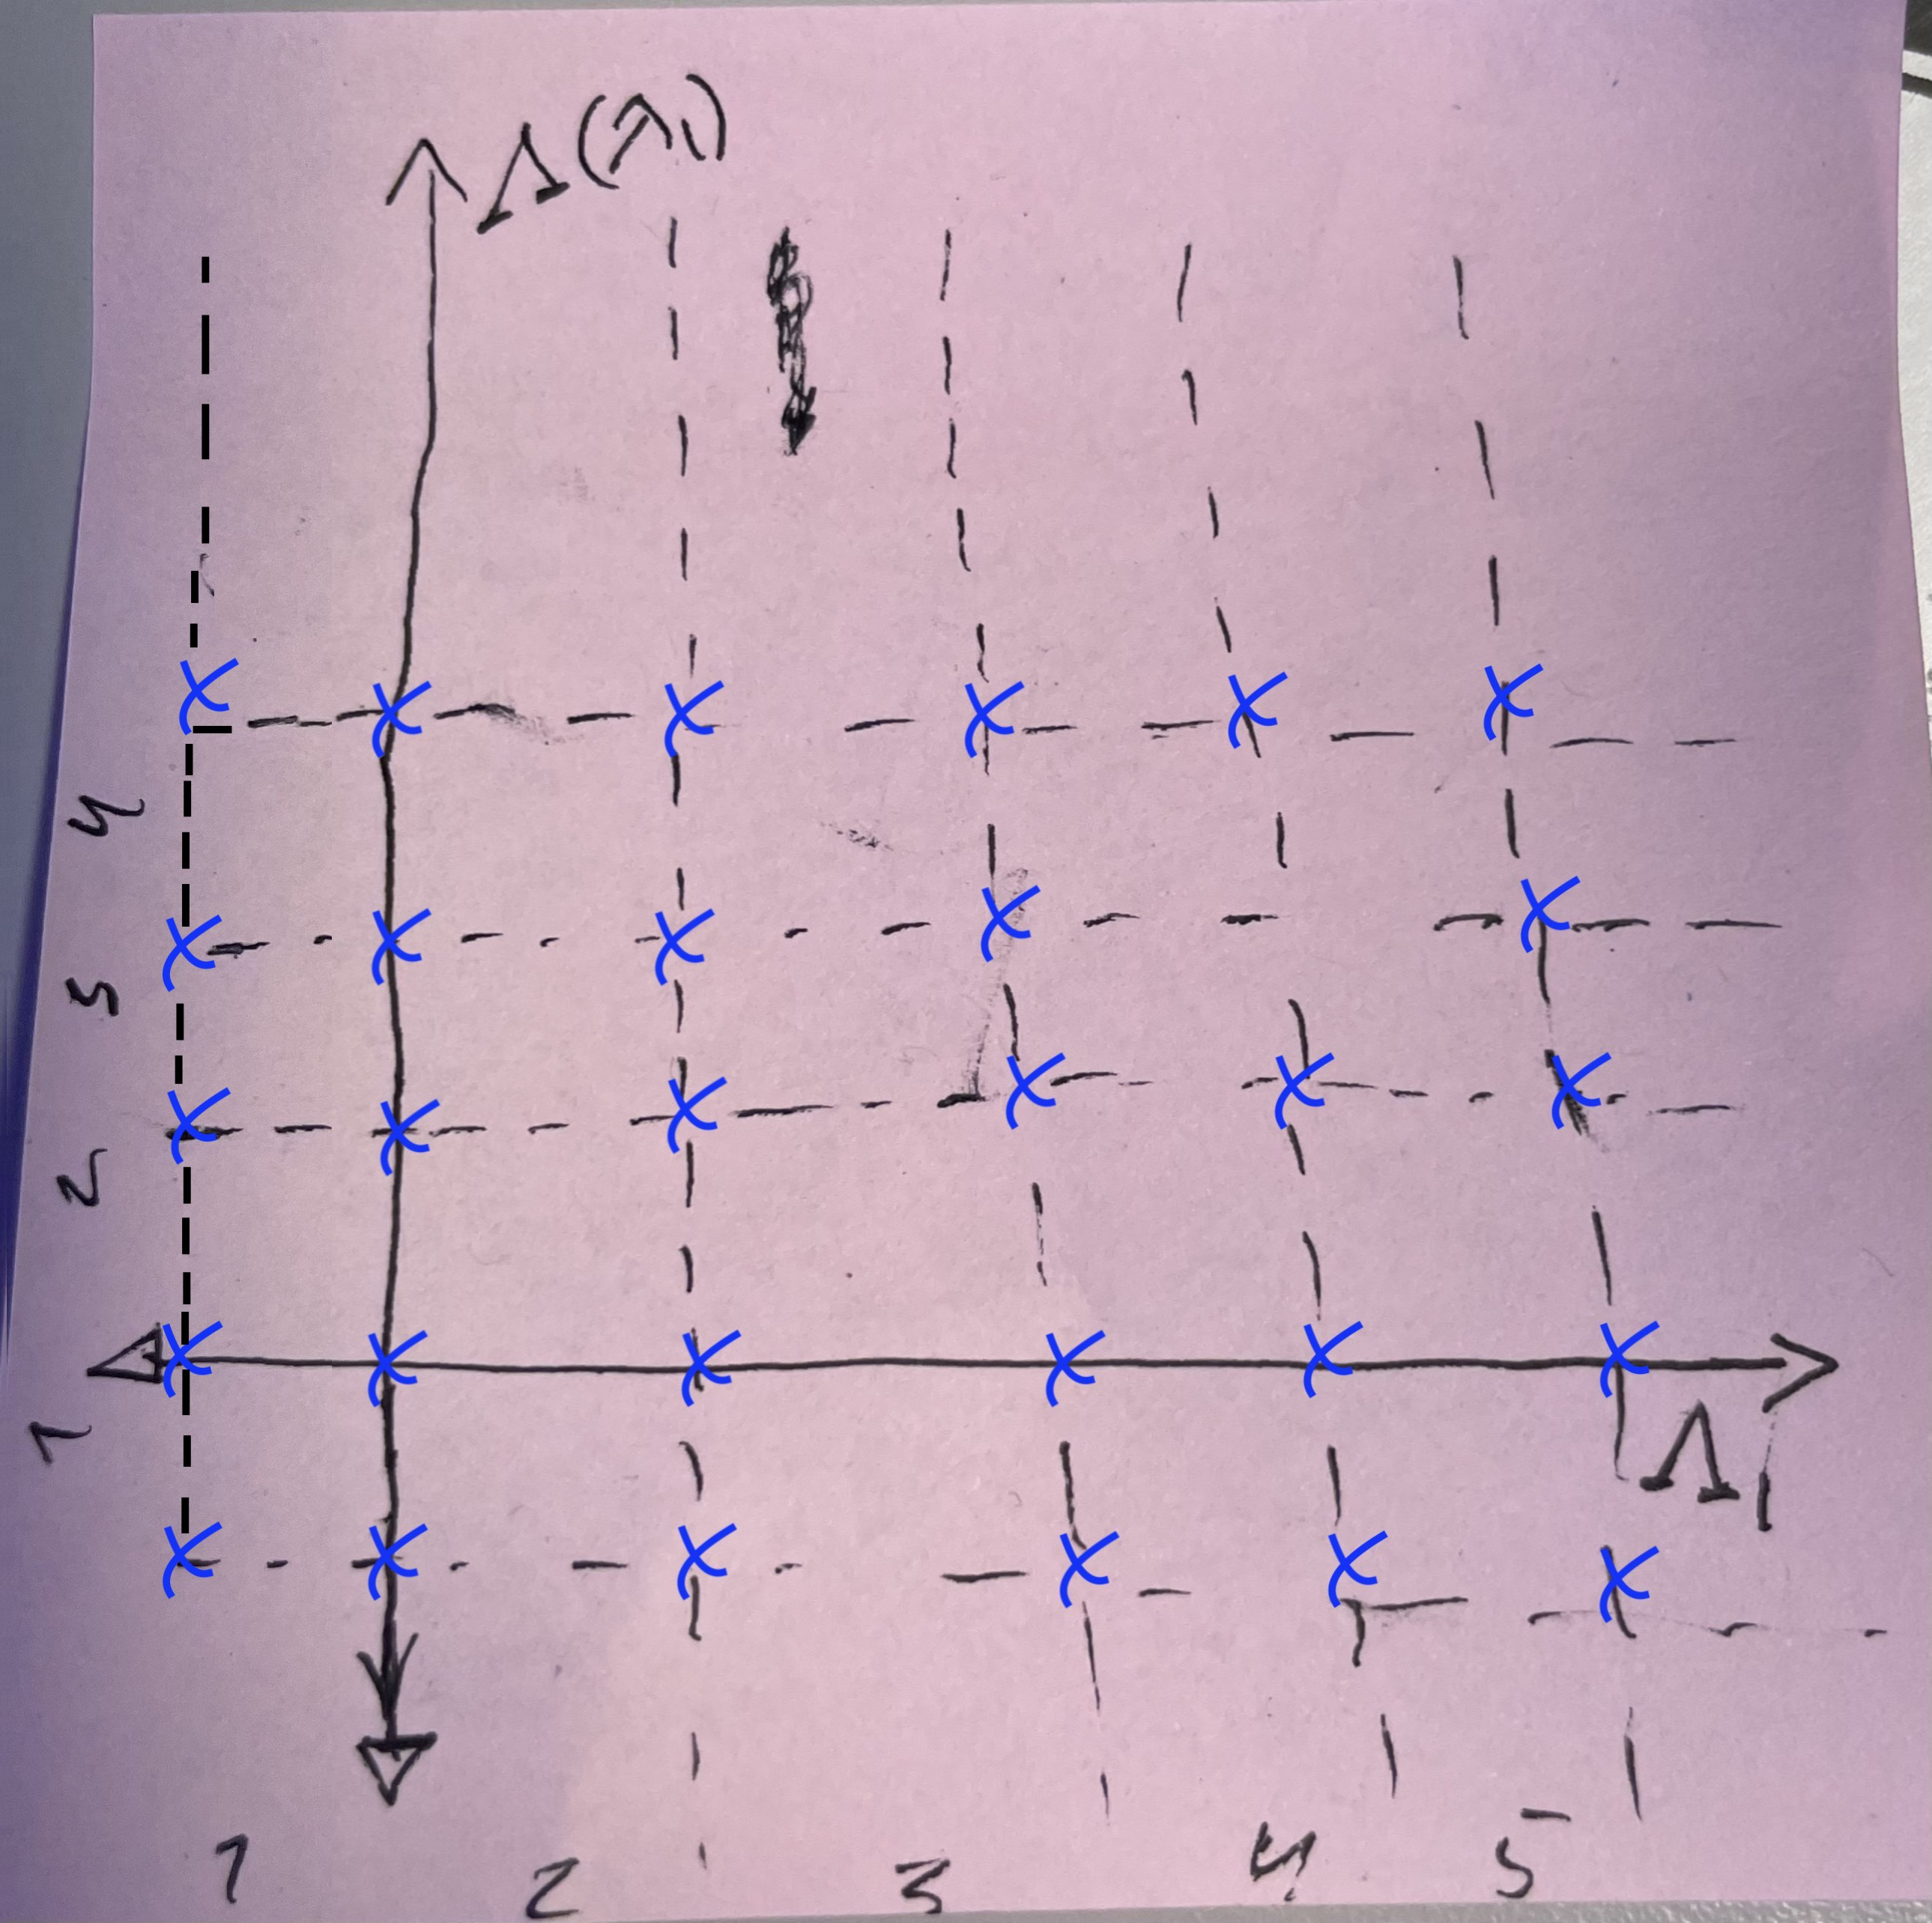
\includegraphics[width=0.9\linewidth]{spec_no_shift.jpg}
        %* Figure 1
        \begin{tikzpicture}[scale=1]
            % Define the tile
            \def\tile{
            \draw[fill=white] (0,0) rectangle (1,1);
            }
            \def\tiletwo{
            %\draw[black, fill=gray!65] (0,0) rectangle (1,1);
            %\draw[black, fill=cyan!65] (0,0) rectangle (1,1);
            \draw[pattern=north east lines, pattern color=MaxCyan4] (0,0) rectangle (1,1);
            }
            
            % Draw the tiling pattern
            % Shifted line, part 1, left and right half tiles 
            \foreach \x in {0}{
                %\draw[cyan, fill=cyan] (\x-0.2,2) rectangle (\x+0.5,3);  % leftmost value to the first square
                \draw[white, pattern=north east lines, pattern color=MaxCyan4] (\x-0.2,2) rectangle (\x+0.5,3); % leftmost value to the first square
            }
            \foreach \x in {6}{
                \draw[white, pattern=north east lines, pattern color=MaxCyan4] (\x+0.2,2) rectangle (\x-0.5,3);
                %\draw[gray!65, fill=cyan!65] (\x+0.2,2) rectangle (\x-0.5,3);  % rightmost value to the last square
            }
            % part 2, whole tiles in the middle
            % must be after the above code in order to get black lines at the correct spots
            \foreach \y in {2}{
                \foreach \x in {0,1,2,3,4}{
                    \pgfmathsetmacro{\shiftX}{\x+0.5} % Set horizontal shift
                    \pgfmathsetmacro{\shiftY}{\y}
                    \begin{scope}[shift={(\shiftX,\shiftY)}]
                        \tiletwo
                    \end{scope}
                }
            }
            % Everything else
            \foreach \y in {0,1,3,4}{
                \foreach \x in {0,1,2,3,4,5}{
                    \pgfmathsetmacro{\shiftX}{\x} % Set horizontal shift
                    \pgfmathsetmacro{\shiftY}{\y}
                    \begin{scope}[shift={(\shiftX,\shiftY)}]
                        \tile
                    \end{scope}
                }
            }
            % get the outline grid 
            



% small black lines at the left and right
\foreach \y in {0,1,2,3,4,5}{
    \draw (0-0.2,\y) -- (0,\y);  % Left
    \draw (6,\y) -- (6+0.2,\y);  % Right
    
}

% small black lines at the top and bottom
\foreach \x in {0,1,2,3,4,5,6}{
    \draw (\x,0-0.2) -- (\x,0);  % Top
    \draw (\x,5) -- (\x,5+0.2);  % Bottom
}
        \end{tikzpicture}
        %* —————————————————
        \caption{Single row shift}
        \label{fig:single_shift_horizontal_tiling}
    \end{subfigure}\quad
    \begin{subfigure}{.47\textwidth}
        \centering
        %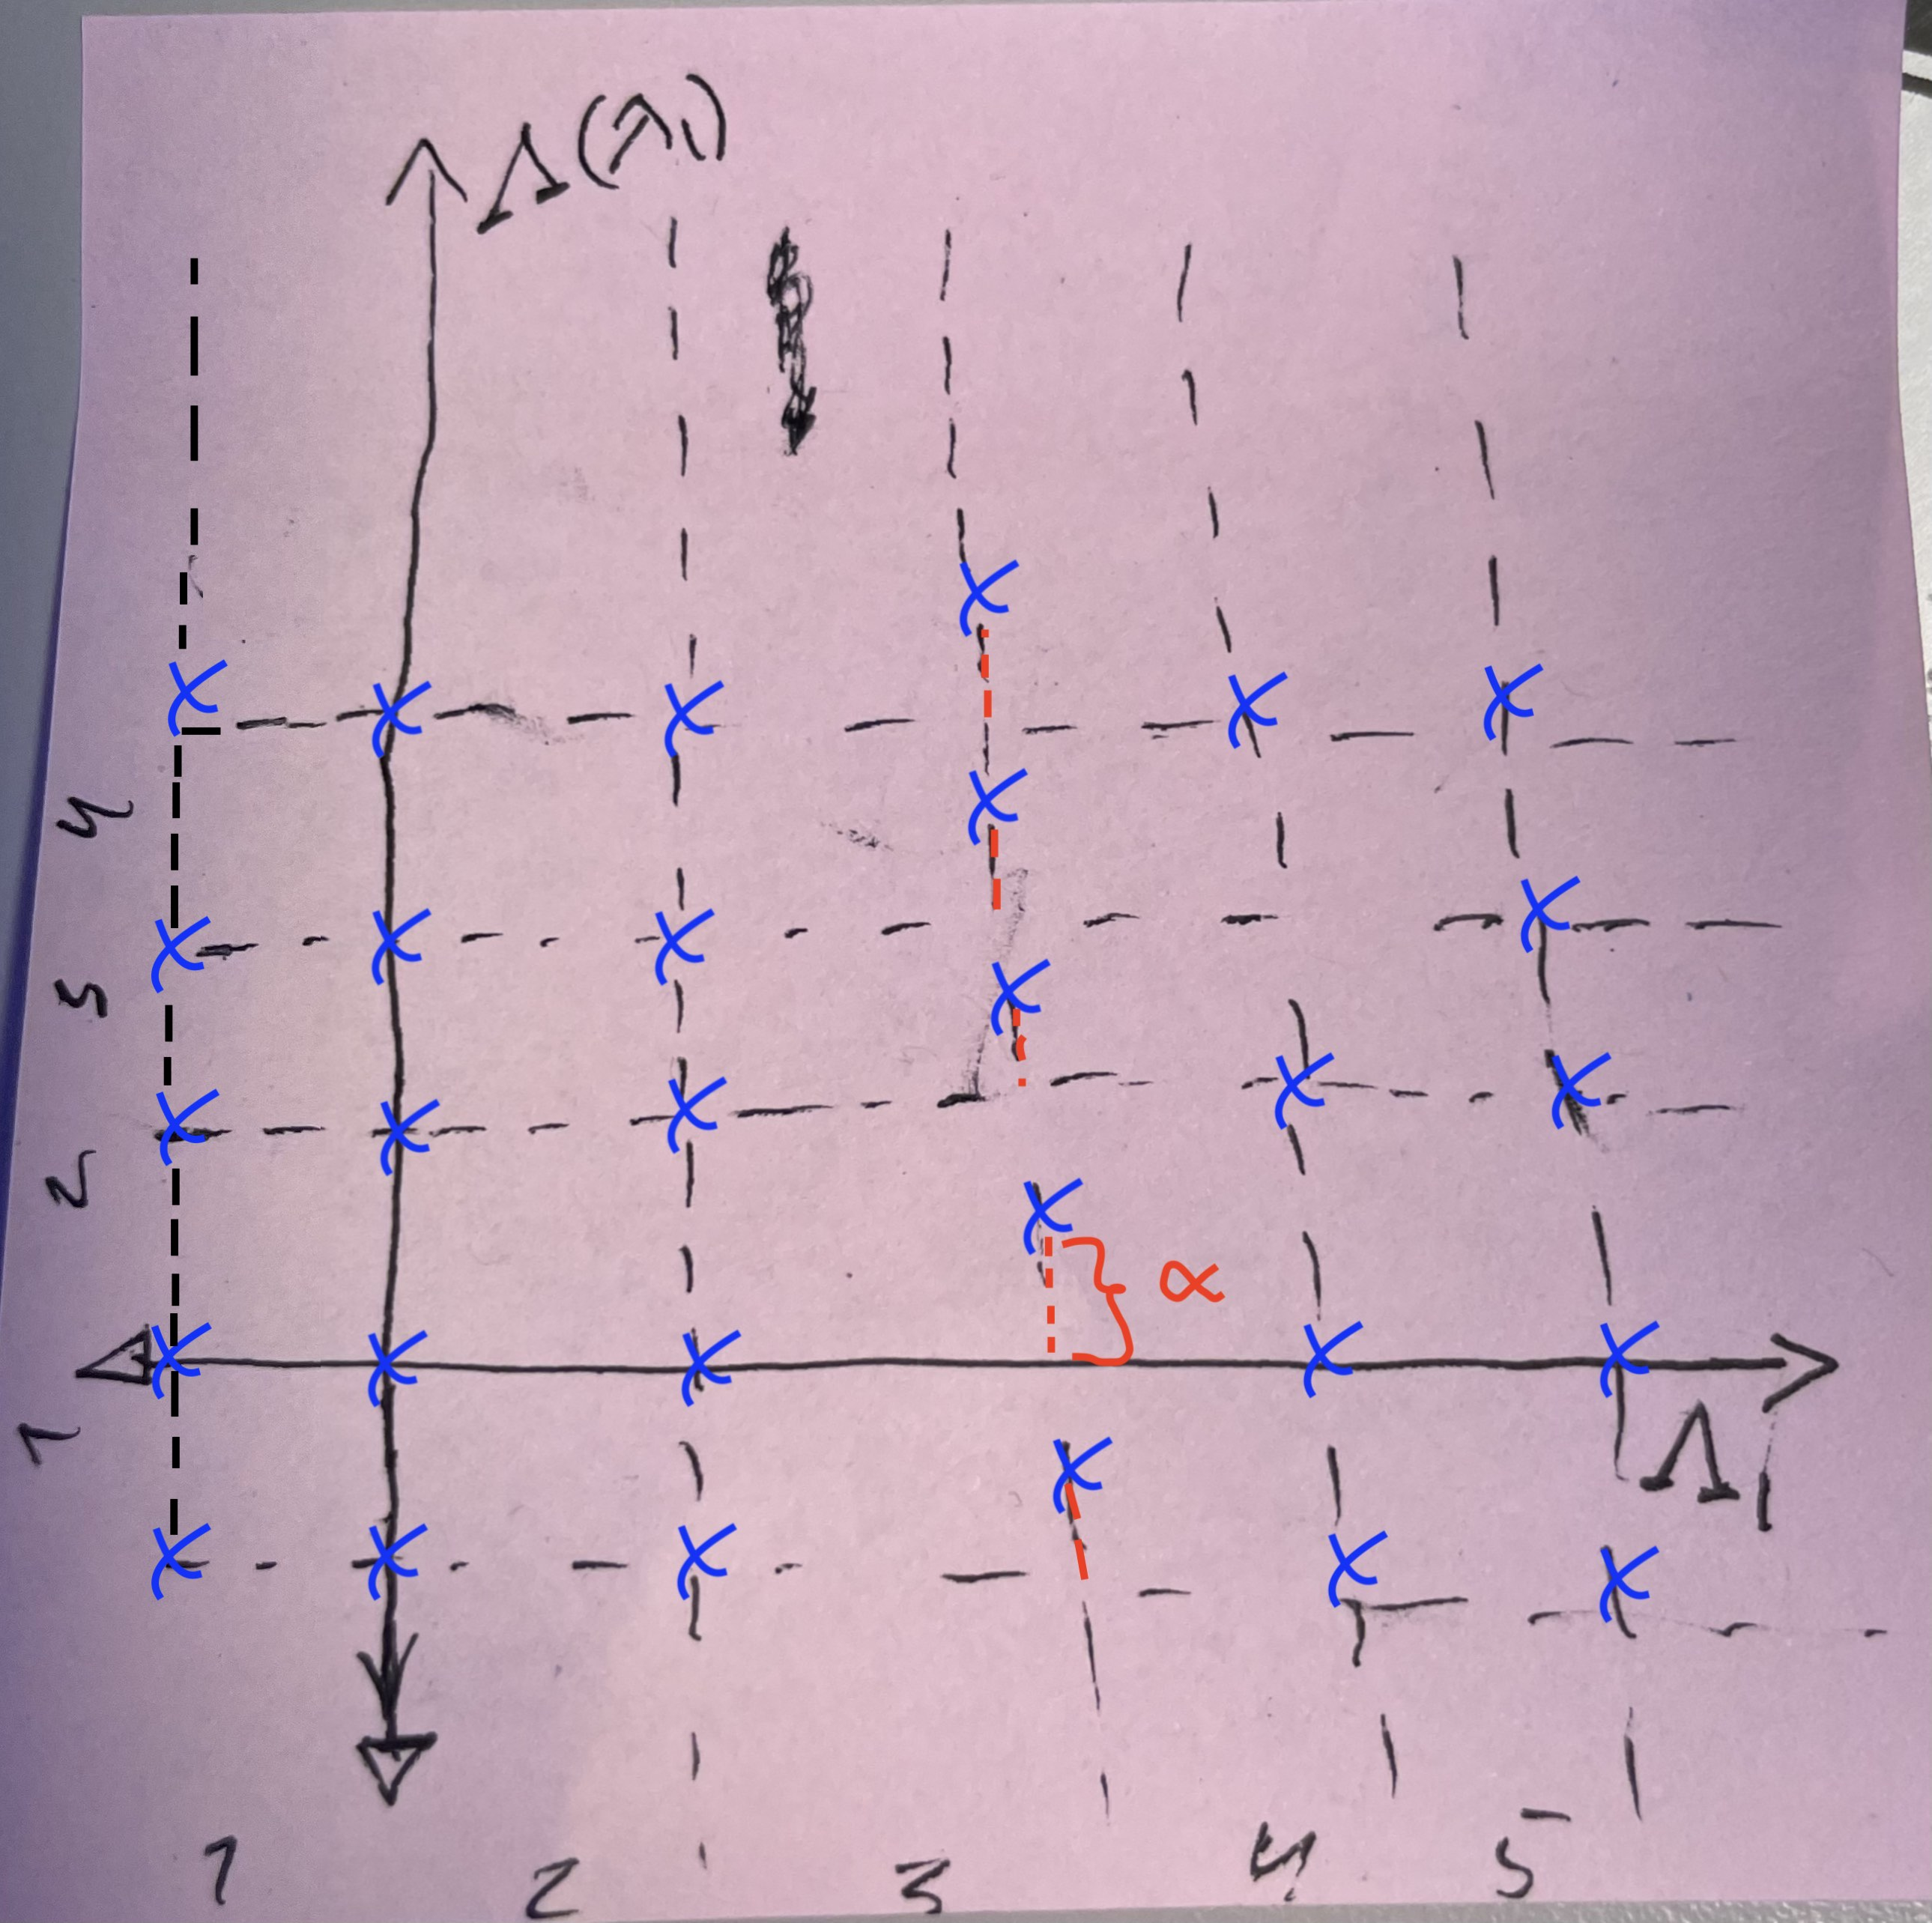
\includegraphics[width=0.9\linewidth]{spec_single_shift.jpg}
        %* Figure 2
        \begin{tikzpicture}[scale=1]
            % Define the tile
            \def\tile{
            \draw[fill=white] (0,0) rectangle (1,1);
            }
            \def\tiletwo{
            %\draw[fill=gray!65] (0,0) rectangle (1,1);
            %\draw[fill=YellowOrange] (0,0) rectangle (1,1);
            \draw[pattern=north east lines, pattern color=MaxOrange] (0,0) rectangle (1,1);
            }
            
            % Draw the tiling pattern
            % Shifted line, part 1, left and right half tiles 
            \foreach \y in {0}{
                %\draw[YellowOrange, fill=YellowOrange] (2,\y-0.2) rectangle (3,\y+0.5);
                \draw[white, pattern=north east lines, pattern color=MaxOrange] (2,\y-0.2) rectangle (3,\y+0.5);
                %\draw[orange!75, fill=orange!75] (2,\y-0.2) rectangle (3,\y+0.5);
            }
            \foreach \y in {5}{
                %\draw[YellowOrange, fill=YellowOrange] (2,\y+0.2) rectangle (3,\y-0.5);
                \draw[white, pattern=north east lines, pattern color=MaxOrange] (2,\y+0.2) rectangle (3,\y-0.5);
                %\draw[gray!65, fill=orange] (2,\y+0.2) rectangle (3,\y-0.5);
            }
            % part 2, whole tiles in the middle
            % must be after the above code in order to get black lines at the correct spots
            \foreach \x in {2}{
                \foreach \y in {0,1,2,3}{
                    \pgfmathsetmacro{\shiftX}{\x} % Set horizontal shift
                    \pgfmathsetmacro{\shiftY}{\y+0.5}
                    \begin{scope}[shift={(\shiftX,\shiftY)}]
                        \tiletwo
                    \end{scope}
                }
            }
            % Everything else
            \foreach \x in {0,1,3,4,5}{
                \foreach \y in {0,1,2,3,4}{
                    \pgfmathsetmacro{\shiftX}{\x} % Set horizontal shift
                    \pgfmathsetmacro{\shiftY}{\y}
                    \begin{scope}[shift={(\shiftX,\shiftY)}]
                        \tile
                    \end{scope}
                }
            }
            % get the outline grid 
            



% small black lines at the left and right
\foreach \y in {0,1,2,3,4,5}{
    \draw (0-0.2,\y) -- (0,\y);  % Left
    \draw (6,\y) -- (6+0.2,\y);  % Right
    
}

% small black lines at the top and bottom
\foreach \x in {0,1,2,3,4,5,6}{
    \draw (\x,0-0.2) -- (\x,0);  % Top
    \draw (\x,5) -- (\x,5+0.2);  % Bottom
}
        \end{tikzpicture}
        %* —————————————————
        \caption{Single column shift}
        \label{fig:single_shift_vertical_tiling}
    \end{subfigure}\\
    \begin{subfigure}{.47\textwidth}
        \centering
        %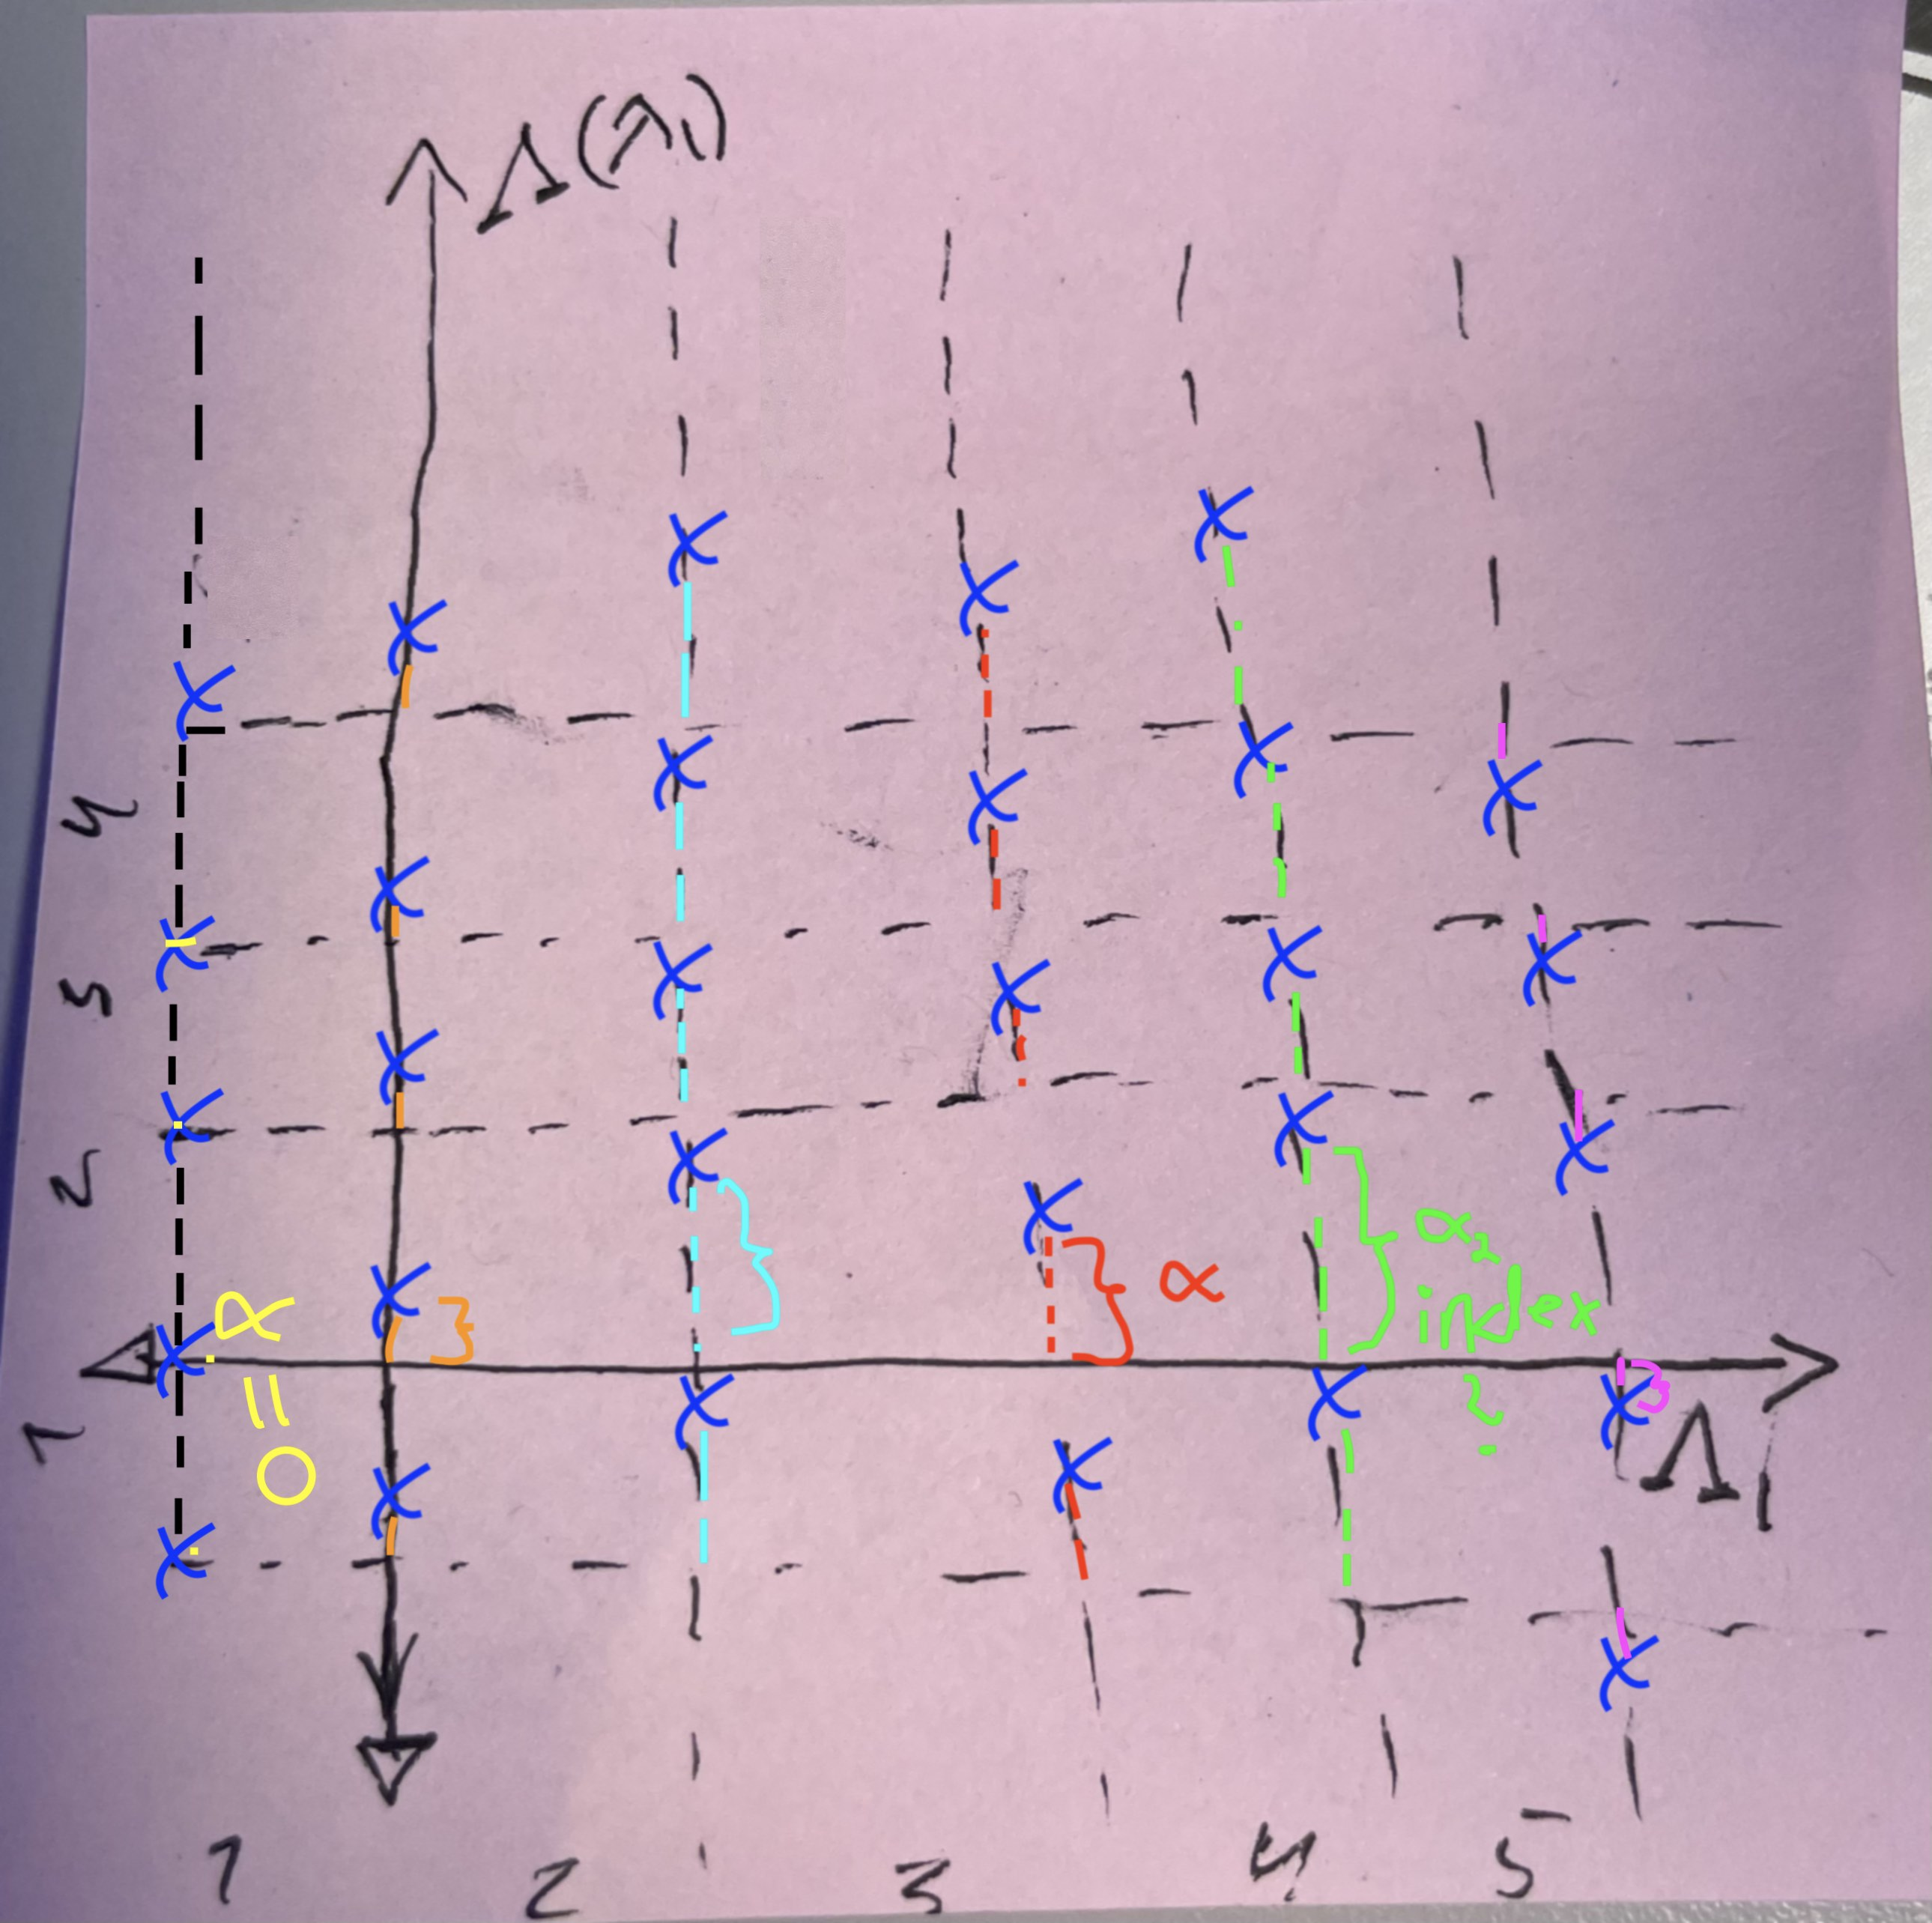
\includegraphics[width=0.9\linewidth]{multiple_shift_left_zero.jpg}
        %* Figure 3
        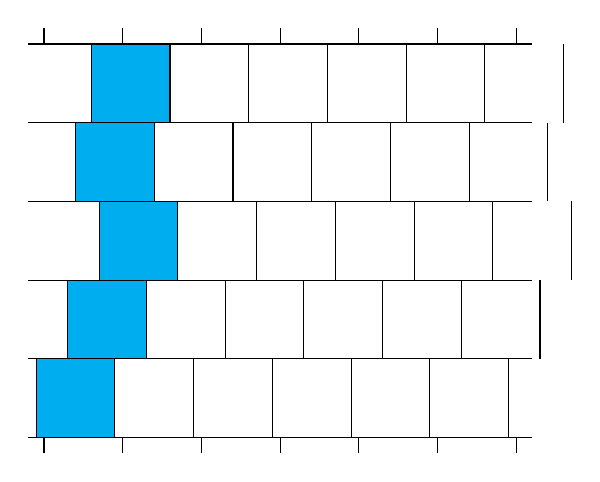
\begin{tikzpicture}[scale=1]
            % Define the tile
            \def\tile{
            % Draw the unit square
            \draw[fill=white] (0,0) rectangle (1,1);
            }
            \def\tiletwo{
            %\draw[fill=gray!65] (0,0) rectangle (1,1);
            \draw[fill=cyan] (0,0) rectangle (1,1);
            }

            % Shift list
            \def\BetaMinOne{-0.1}
            \def\BetaZero{0.3}
            \def\BetaOne{0.7}
            \def\BetaTwo{0.4}
            \def\BetaThree{0.6}
            
            % Draw the tiling pattern
            \foreach \x in {0,1,2,3,4}{
                \foreach \y in {0,1,2,3,4}{
                    \ifnum\y=0
                        \pgfmathsetmacro{\shiftX}{\x + \BetaMinOne}
                        \pgfmathsetmacro{\shiftY}{\y}
                        \pgfmathsetmacro{\shiftSingle}{\BetaMinOne}
                    \fi
                    \ifnum\y=1
                        \pgfmathsetmacro{\shiftX}{\x + \BetaZero}
                        \pgfmathsetmacro{\shiftY}{\y}
                        \pgfmathsetmacro{\shiftSingle}{\BetaZero}
                    \fi
                    \ifnum\y=2
                        \pgfmathsetmacro{\shiftX}{\x + \BetaOne} 
                        \pgfmathsetmacro{\shiftY}{\y} 
                        \pgfmathsetmacro{\shiftSingle}{\BetaOne}
                    \fi
                    \ifnum\y=3
                        \pgfmathsetmacro{\shiftX}{\x + \BetaTwo}
                        \pgfmathsetmacro{\shiftY}{\y}
                        \pgfmathsetmacro{\shiftSingle}{\BetaTwo}
                    \fi
                    \ifnum\y=4
                        \pgfmathsetmacro{\shiftX}{\x + \BetaThree}
                        \pgfmathsetmacro{\shiftY}{\y}
                        \pgfmathsetmacro{\shiftSingle}{\BetaThree}
                    \fi
                    % Drawing the left half-cubes
                    \ifnum\x=0
                        \draw[white, fill=white](\x-0.2,\y) rectangle (\x+\shiftSingle,\y+1);
                    \fi
                    % Drawing the right half-cubes
                    \ifnum\x=4
                        \ifthenelse{\lengthtest{\shiftSingle pt > 0.2 pt}}{
                            \draw[white] (\x+2+\shiftSingle,\y+1) -- (\x+2+\shiftSingle,\y);  % Right line
                        }{
                            \draw[black] (\x+2+\shiftSingle,\y+1) -- (\x+2+\shiftSingle,\y);  % Right line
                        }
                        %\draw[black] (\x+1,\y) -- (\x,\y+2);  % Left line
                        %\draw[black] (\x+2+\shiftSingle,\y) -- (\x+2+\shiftSingle,\y+1);  % Top
                        %\draw[black] (\x+1+\shiftSingle,\y+1) -- (\x+1+\shiftSingle,\y);  % Bottom line
                    \fi
                    % Drawing the rest of the middle cubes
                    \begin{scope}[shift={(\shiftX,\shiftY)}]
                        \tile % Draw the tile
                    \end{scope}
                    % Drawing a new line of shifted colored cubes on top at the first row
                    \ifnum\x=0
                    \begin{scope}[shift={(\shiftX,\shiftY)}]
                        \tiletwo
                    \end{scope}
                    \fi
                }   
            }
            % get the outline grid 
            % small black lines at the left and right
            \foreach \y in {0,1,2,3,4,5}{
                %\draw (0-0.2,\y) -- (0,\y);  % Left
                %\draw (6,\y) -- (6+0.2,\y);  % Right
                \draw (0-0.2,\y) -- (6+0.2,\y);  % Right
            }
            
            % small black lines at the top and bottom
            \foreach \x in {0,1,2,3,4,5,6}{
                \draw (\x,0-0.2) -- (\x,0);  % Top
                \draw (\x,5) -- (\x,5+0.2);  % Bottom
            }
        \end{tikzpicture}
        %* —————————————————
        \caption{Multiple row shifts}
        \label{fig:multiple_shift_horizontal_tiling}
    \end{subfigure}\quad
    \begin{subfigure}{.47\textwidth}
        \centering
        %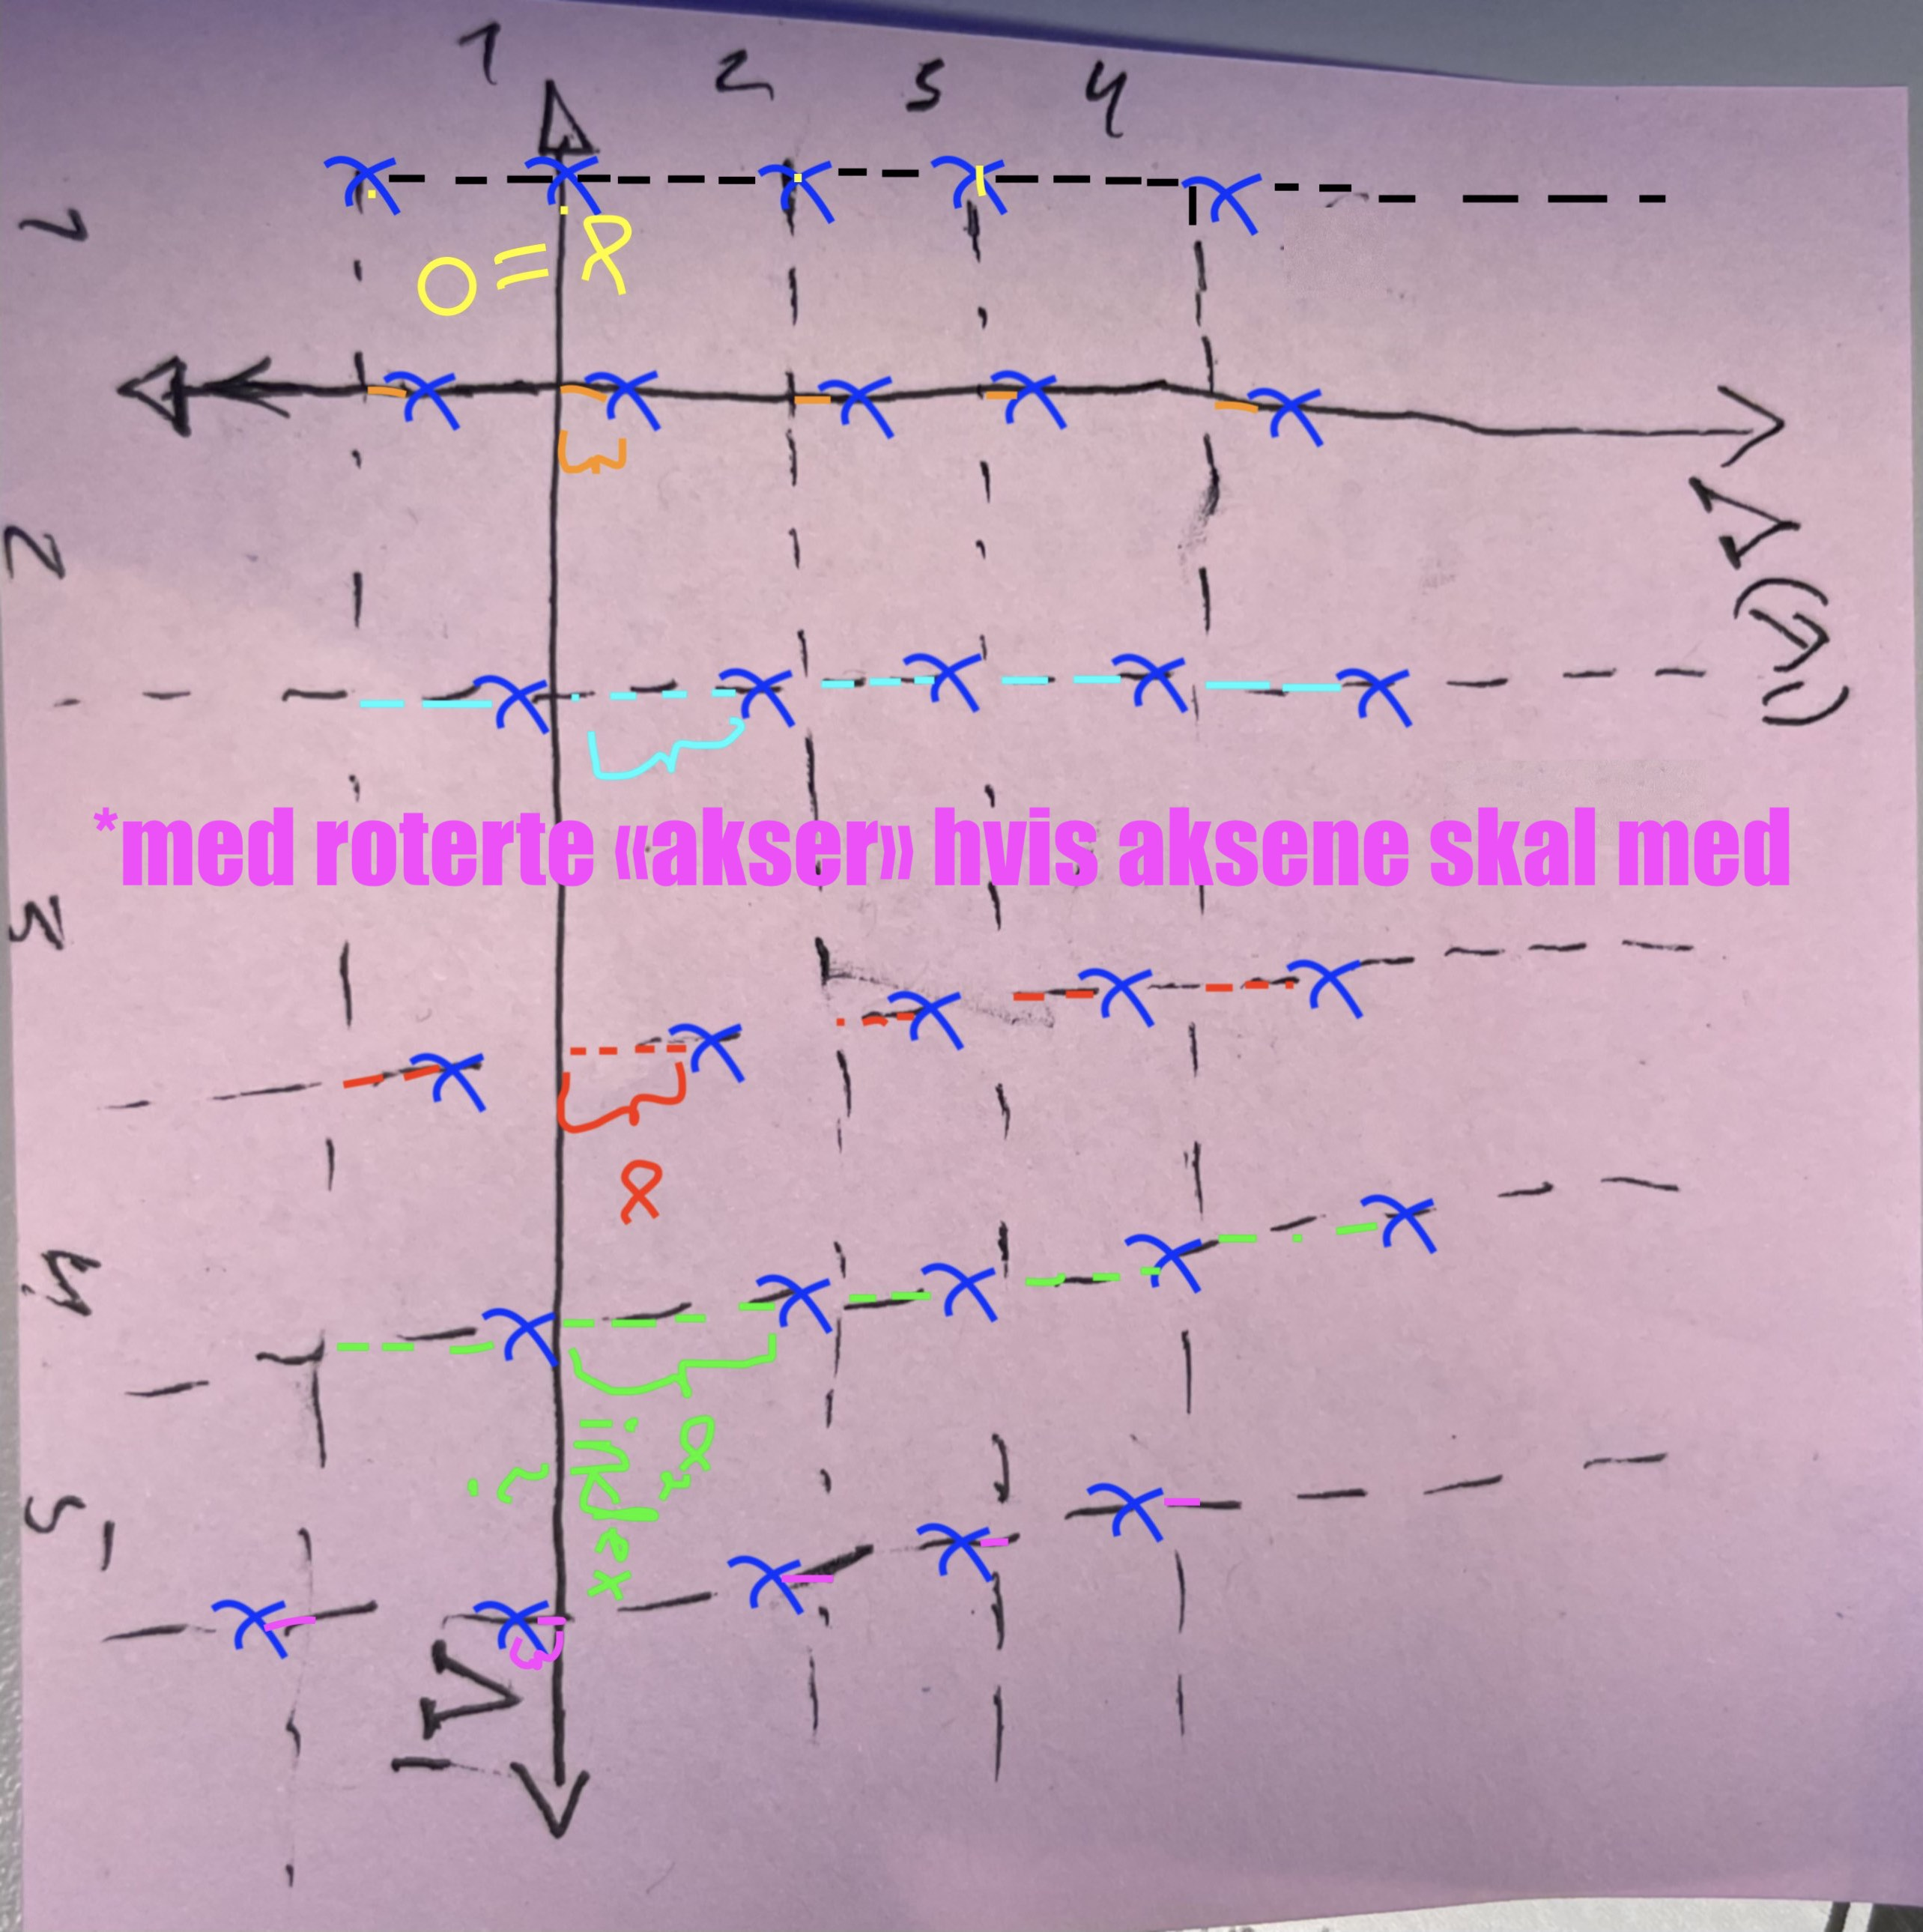
\includegraphics[width=0.9\linewidth]{multiple_shift_left_zero_horizontal.jpg}
        %* Figure 4
        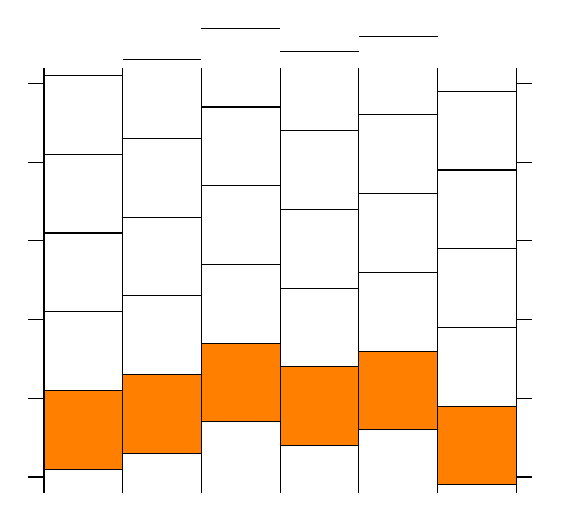
\begin{tikzpicture}[scale=1]
            % Define the tile
            \def\tile{
            % Draw the unit square
            \draw[fill=white] (0,0) rectangle (1,1);
            }
            \def\tiletwo{
            %\draw[fill=gray!65] (0,0) rectangle (1,1);
            \draw[fill=orange] (0,0) rectangle (1,1);
            %\draw[->] (0.5,0) -- (0.5,0.9);  % If arrows from the middle
            }

            % Shift list
            \def\BetaMinOne{0.1}
            \def\BetaZero{0.3}
            \def\BetaOne{0.7}
            \def\BetaTwo{0.4}
            \def\BetaThree{0.6}
            \def\BetaFour{-0.1}

            % Draw the tiling pattern
            \foreach \x in {0,1,2,3,4,5}{
                \foreach \y in {0,1,2,3}{
                    \ifnum\x=0
                        \pgfmathsetmacro{\shiftX}{\x}
                        \pgfmathsetmacro{\shiftY}{\y + \BetaMinOne}
                        \pgfmathsetmacro{\shiftSingle}{\BetaMinOne}
                    \fi
                    \ifnum\x=1
                        \pgfmathsetmacro{\shiftX}{\x}
                        \pgfmathsetmacro{\shiftY}{\y + \BetaZero}
                        \pgfmathsetmacro{\shiftSingle}{\BetaZero}
                    \fi
                    \ifnum\x=2
                        \pgfmathsetmacro{\shiftX}{\x} 
                        \pgfmathsetmacro{\shiftY}{\y + \BetaOne} 
                        \pgfmathsetmacro{\shiftSingle}{\BetaOne}
                    \fi
                    \ifnum\x=3
                        \pgfmathsetmacro{\shiftX}{\x}
                        \pgfmathsetmacro{\shiftY}{\y + \BetaTwo}
                        \pgfmathsetmacro{\shiftSingle}{\BetaTwo}
                    \fi
                    \ifnum\x=4
                        \pgfmathsetmacro{\shiftX}{\x}
                        \pgfmathsetmacro{\shiftY}{\y + \BetaThree}
                        \pgfmathsetmacro{\shiftSingle}{\BetaThree}
                    \fi
                    \ifnum\x=5
                        \pgfmathsetmacro{\shiftX}{\x}
                        \pgfmathsetmacro{\shiftY}{\y + \BetaFour}
                        \pgfmathsetmacro{\shiftSingle}{\BetaFour}
                    \fi
                    % Drawing the bottom half-cubes
                    \ifnum\y=0
                        \draw[white, fill=white](\x,\y-0.2) rectangle (\x+1,\y+\shiftSingle);
                    \fi
                    % Drawing the top half-cubes
                    \ifnum\y=3
                        \ifthenelse{\lengthtest{\shiftSingle pt > 0.2 pt}}{
                            \draw[white] (\x,\y+2+\shiftSingle) -- (\x+1,\y+2+\shiftSingle);  % Top
                        }{
                        \draw[black] (\x,\y+2+\shiftSingle) -- (\x+1,\y+2+\shiftSingle);  % Top
                        }
                        \draw[black] (\x,\y+1) -- (\x,\y+2);  % Left line
                        \draw[black] (\x+1,\y+2) -- (\x+1,\y+1);  % Right line
                        \draw[black] (\x+1,\y+1+\shiftSingle) -- (\x,\y+1+\shiftSingle);  % Bottom line
                        %\draw[red, fill=red](\x,\y+1) rectangle (\x+1,\y+2);
                    \fi
                    % Drawing the rest of the middle cubes
                    \begin{scope}[shift={(\shiftX,\shiftY)}]
                        \tile
                    \end{scope}
                    % Drawing a new line of shifted colored cubes on top at the first row
                    \ifnum\y=0
                        \begin{scope}[shift={(\shiftX,\shiftY)}]
                            \tiletwo
                        \end{scope}
                    \fi
                }  
            }
            % get the outline grid 
            % small black lines at the left and right
            \foreach \y in {0,1,2,3,4,5}{
                \draw (0-0.2,\y) -- (0,\y);  % Left
                \draw (6,\y) -- (6+0.2,\y);  % Right
            }
            % small black lines at the top and bottom
            \foreach \x in {0,1,2,3,4,5,6}{
                %\draw (\x,0-0.2) -- (\x,0);  % Top
                %\draw (\x,5) -- (\x,5+0.2);  % Bottom
                \draw (\x,0-0.2) -- (\x,5+0.2);  % Shift only in the vertical direction, therefore only one line
            }
        \end{tikzpicture}
        %* —————————————————
        \caption{Multiple column shifts}
        \label{fig:multiple_shift_vertical_tiling}
    \end{subfigure}
    \caption{Illustration of four tiling pairs for $\brac{I^2,\Lambda}$ covering $\R^2$. The cyan and orange colors represent shifts in the horizontal and vertical direction, respectively. The dashed line pattern in \cref{fig:single_shift_horizontal_tiling,fig:single_shift_vertical_tiling} highlights the single row or column which is shifted, and the filled cubes in \cref{fig:multiple_shift_horizontal_tiling,fig:multiple_shift_vertical_tiling} highlights the different shifts used for each row or column. Note that if this were a lattice tiling, all the cyan-filled or orange-filled squares would be on the same vertical or horizontal line, respectively.}
    \label{fig:tiling_figures}
\end{figure}

%\extractcolorspecs{Cyan}{\myColorModel}{\myColor} orange is \myColor\ in model %\myColorModel



\clearpage
\SigridComment{Gammelt, med gammel struktur}
\begin{definition}[Tiling set]
    Let $\Omega \subset \R^d$ be a subset with nonzero measure, and consider a set $\Lambda \subset \R^d$. If $T(\Lambda)$ cover $\R^d$ up to measure zero, and if all intersections of 
    \begin{equation*}  %* NON OVERLAPPING
        (\Omega+\lambda) \cap (\Omega+\lambda')
    \end{equation*}
    for $\lambda\neq \lambda'$ in $\Lambda$ have measure zero, then $\Omega$ is called a \emph{tile}, and $\Lambda$ is called a \emph{tiling set} for $\Omega$. We say that $(\Omega, \Lambda)$ is a \emph{tiling pair}. 
\end{definition}
\begin{definition}
    Let $\Omega \subset \R^d$ be a subset with nonzero measure, and consider a set $\Lambda \subseteq \R^d$. If the following two conditions are satisfied, then $\Omega$ is called a \emph{tile}, and $\Lambda$ is called a \emph{tiling set} for $\Omega$. We say that $(\Omega, \Lambda)$ is a \emph{tiling pair}. 
    \begin{itemize}
        \item If $T(\Lambda)$ cover $\R^d$ up to measure zero. That is,  %* Cover the whole space
        \begin{equation*}
            \bigcup_{\lambda \in \Lambda} (\Omega + \lambda) = \R^d
        \end{equation*}
        \item If all intersections of $(\Omega+\lambda) \cap (\Omega+\lambda')$ for $\lambda\neq \lambda'$ in $\Lambda$ have measure zero. %* Mutually NON-OVERLAPPING 
    \end{itemize}
\end{definition}


\section{Tiling sets for the n-cube}
\section{The unit cube in dimension one / Tilings in dimension one}
%* Hva vet vi om tilings i en dimensjon for unit cube, jo der har vi bare et alternativ og det er det samme alternativet som for spectral Set
%* paper + andre kilder, søke opp
In dimension one, the unit cube is simply the unit interval $I=\bras{0,1}$.
\begin{theorem}  %* Bruker alle elementene i T for å flytte på I, da dekker vi hele $\R$.  
    Let $\Omega = I$. If $T=\Z$, then $T$ is a tiling set for $I$.
\end{theorem}

\begin{proof}
    It is clear that
    \begin{align*}
        %\bigcup_{\lambda\in \Z} (I + \lambda) &= \bigcup_{\lambda\in \Z} \braq{\omega + \lambda : \omega \in I}\\
        \bigcup_{\lambda\in \Z} (I + \lambda) &= \dots (I-1) \cup (I-0) \cup (I+1) \dots\\ 
        &= \dots [-1,0] \cup [0,1] \cup [1,2] \dots\\
        &= \R
    \end{align*}
    and that 
    \begin{align*}
        \mesMed{\R \setminus \bigcup_{\lambda\in \Z} (I + \lambda) } = \mesMed{\emptyset} = 0.
    \end{align*}
    This shows that the set of translates $T(\Lambda)$ covers $\R$ up to measure zero. 
    
    Now take $\lambda,\lambda' \in \Z$. If $\lambda = \lambda'$ we have that
    \begin{equation*}
        \mes{(I+\lambda) \cap (I+\lambda')} = \mes{(I+\lambda)} = (1+\lambda) - (0+\lambda) = 1.
    \end{equation*}
    And if $\lambda \neq \lambda'$ we have that 
    \begin{equation*}
        \mes{(I+\lambda) \cap (I+\lambda')} = \mes{\emptyset} = 0,
    \end{equation*}
    showing that the cubes are non-overlapping for all distinct $\lambda , \lambda' \in T$. 
\end{proof}


\subsection{The unit cube in higher dimensions / Tilings in higher dimensions}
-> når det er større en 1 har vi flere muligheter

-> en begrensing legges av Kellers theorem, 


\SigridComment{END}



% ! Def tiling
%\begin{definition}[Tiling set]
%    Let $\Omega \subset \mathbb{R}^d$ be a subset with nonzero measure, and consider a set $T \subseteq \mathbb{R}^d$. If the set of translates ${}$$\{\Omega+l: l\in T\}$ cover $\mathbb{R^d}$ up to measure zero, and if all intersections $(\Omega+l) \cap (\Omega+l')$  for $l\neq l'$ in $L$ have measure zero, then $\Omega$ is called a \emph{tile}, and $T$ is called a \emph{tiling set} for $\Omega$. We say that $(\Omega, T)$ is a \emph{tiling pair}. 
%\end{definition}

%In other words, the shifts $\Omega + T$ constitute a \emph{measuredisjoint covering} of $\mathbb{R}^d$, and we can say that $\Omega$ \emph{tiles} $\mathbb{R}^d$ \emph{by translation}, or that $\Omega+T$ is a \emph{tiling} of $\mathbb{R}^d$.


% Fuglede’s spectral set conjecture. Let $\Omega$􏱁 be a set in $\mathbb{R}^d$ with positive and finite Lebesgue measure. Then 􏱁$\Omega$ is a spectral set if and only if $\Omega$􏱁 tiles $\mathbb{R}^d$ by translation.

% An equivalent restatement of Fuglede was presented in Jorgen/Pedersen. 

% Let $\Omega \subset \mathbb{R}^d$ have positive and finite Lebesgue measure. Then $\Omega$ is a spectral set if and only if $\Omega$ is a tile, i.e., there exists a set $\Lambda$ so that $(\Omega, \Lambda)$ is a spectral pair if and only if there exists a set $\Lambda^{\prime}$ so that $\left(\Omega, \Lambda^{\prime}\right)$ is a tiling pair.

%with the following dual conjectures.

% Conjecture 1.3: Let $\Lambda \subset \mathbb{R}^d$. Then $\Lambda$ is a spectrum if and only if $\Lambda$ is a tiling set, i.e., there exists a set $\Omega$ so that $(\Omega, \Lambda)$ is a spectral pair if and only if there exists a set $\Omega^{\prime}$ so that $\left(\Omega^{\prime}, \Lambda\right)$ is a tiling pair.

% Conjecture 1.4: Let $\Lambda \subset \mathbb{R}^d$. Then $\left(I^d, \Lambda\right)$ is a spectral pair if and only if $\left(I^d, \Lambda\right)$ is a tiling pair.

%When  $\Omega = I^d$ the connection between tiles and spectrum is more direct than for other examples of sets $\Omega$. As shown in sigrid_note:lagarias_reeds_wang and Spectral and tiling properties of the unit cube_ALEX IOSEVICH AND STEEN PEDERSEN it is possible to classify all spectra by showing that $\Lambda$ is a spectrum for the unit cube $I^d$, if and only if $I^d$ tiles $\mathbb{R}^d$ by $\Lambda$-translates.






\end{document}


